\chapter{Resultados e Discussões} \label{cap:resultados}

Neste capítulo são apresentados os resultados obtidos pela execução da metodologia proposta no \autoref{cap:desenvolvimento} e as discussões acerca dos mesmos. A análise dos resultados é realizada com base nos cenários de ataques cibernéticos apresentados na \autoref{sec:attacks}, com o intuito de avaliar a robustez das redes industriais OPC UA e a variação no desempenho dos componentes ao serem submetidos a tais cenários. Para organização das informações, os resultados são divididos em seções que correspondem a cada etapa da metodologia apresentada.

Como regra geral, espera-se fornecer informações valiosas sobre vulnerabilidades potenciais que podem ser expostas durante o processo de experimentação. Estas prospecções, caso confirmadas, auxiliam em avanços futuros do protocolo OPC UA e de sistemas IACS, fortalecendo ainda mais a robustez destes e resistência contra ameaças cibernéticas em constante evolução.

\section{Implementação da Bancada Experimental} \label{sec:impl-bancada}

A \autoref{fig:banc} apresenta a bancada experimental para ensaios de segurança cibernética, composta por um servidor OPC UA, um cliente OPC UA e um \textit{firewall} industrial. O servidor OPC UA é responsável por disponibilizar os dados de processo e controlar o sistema de automação industrial, enquanto o cliente OPC UA é responsável por acessar e visualizar esses dados. O \textit{firewall} industrial é utilizado para monitorar e controlar o tráfego de dados entre o servidor e o cliente, garantindo a segurança da rede.

\begin{figure}[htbp!]
    \caption{\label{fig:banc}Bancada experimental para ensaios de segurança cibernética}
    \begin{center}
        \includegraphics[width=0.5\textwidth]{USPSC-img/cyberkit2.png}
    \end{center}
    \legend{Fonte: elaborada pelo autor.}
\end{figure}

\section{Aquisição dos Dados nos Cenários de Ataques Cibernéticos} \label{sec:exec-attacks}

No passo da metodologia apresentado pela \autoref{sec:aquisicao}, coloca-se a bancada em operação de acordo com os cenários especificados (\autoref{tab:attacks}), aciona-se o sistema de medição, nas quais são realizadas aquisição do tráfego da rede e do desempenho do hospedeiro do servidor OPC UA, e efetua-se os respectivos ataques. Os dados de processa da rede OPC UA são coletados por 60 segundos para cada cenário.

A \autoref{tab:carac-cenarios} apresenta um resumo detalhado das características do tráfego da rede e desempenho em cada cenário de ataque e comunicação normal em redes OPC UA industriais.

\begin{table}[htbp!]
    \centering
    \caption{Informações do tráfego da rede e desempenho do hospedeiro em cada cenário}%
    \label{tab:carac-cenarios}
    \begin{tabular}{M{1.5cm}M{3cm}M{2.5cm}M{2.5cm}M{2cm}M{2cm}}
        \toprule
        \textbf{Cenário} & \textbf{\textit{Throughput} médio (kbits/s)} & \textbf{TP\textsuperscript{1} médio (Bytes)} & \textbf{PPS\textsuperscript{2} médio (pacotes/s)} & \textbf{Tráfego OPC UA (\%)} & \textbf{CPU\textsuperscript{3} (\%)} \\
        \toprule
        C1 & 130 & 127 & 128.4 & 28.7 & 7.31 \\
        \midrule
        C2 & 175 & 153 & 142.9 & 34.4 & 8.91 \\
        \midrule
        C3 & 179 & 162 & 138.3 & 31.8 & 9.01 \\
        \midrule
        C4 & 1166 & 965 & 151.1 & 9.2 & 17.16 \\
        \midrule
        C5 & 6824 & 972 & 877.9 & 5.3 & 10.64 \\
        \midrule
        C6 & 6894 & 973 & 885.9 & 8.2 & 10.78 \\
        \midrule
        C7 & 18000 & 60 & 38438.9 & 0.1 & 14.68 \\
        \midrule
        C8 & 12000 & 60 & 26788.9 & 0.1 & 13.23 \\
        \midrule
        C9 & 15000 & 60 & 31278.5 & 0.1 & 14.81 \\
        \midrule
        C10 & 462 & 171 & 337.3 & 72.9 & 9.86 \\
        \midrule
        C11 & 501 & 180 & 348.0 & 71.9 & 11.27 \\
        \midrule
        C12 & 491 & 184 & 334.1 & 69.8 & 11.36 \\
        \midrule
        C13 & 196 & 173 & 141.4 & 33.0 & 7.52 \\
        \midrule
        C14 & 235 & 195 & 151.3 & 35.2 & 9.03 \\
        \midrule
        C15 & 247 & 203 & 152.6 & 32.3 & 9.09 \\
        \midrule
        C16 & 105 & 125 & 105.3 & 33.1 & 6.80 \\
        \midrule
        C17 & 146 & 148 & 123.4 & 33.1 & 7.84 \\
        \midrule
        C18 & 137 & 159 & 107.9 & 33.2 & 7.96 \\
        \midrule
        C19 & 3410 & 43 & 10012.0 & 0.2 & 7.36 \\
        \midrule
        C20 & 3433 & 43 & 9896.4 & 0.2 & 7.97 \\
        \midrule
        C21 & 3432 & 44 & 9854.8 & 0.2 & 7.97 \\
        \midrule
        C22 & 168 & 127 & 166.1 & 32.1 & N/A \\
        \midrule
        C23 & 223 & 154 & 182.4 & 34.5 & N/A \\
        \midrule
        C24 & 219 & 162 & 169.7 & 32.5 & N/A \\
        \midrule
        C25 & 95 & 121 & 98.5 & 28.3 & 7.01 \\
        \midrule
        C26 & 253 & 142 & 222.7 & 17.9 & 7.95 \\
        \midrule
        C27 & 234 & 147 & 199.8 & 17.1 & 8.25 \\
        \bottomrule
        \multicolumn{6}{>{\tiny}l}{\textsuperscript{1} Tamanho do pacote.} \\
        \multicolumn{6}{>{\tiny}l}{\textsuperscript{2} Taxa de pacotes por segundo.} \\
        \multicolumn{6}{>{\tiny}l}{\textsuperscript{3} Processamento do hospedeiro do servidor OPC UA.} \\
    \end{tabular}
    \fonte{elaborada pelo autor.}%
\end{table}

O \textit{throughput} médio e a média do tamanho dos pacotes dos cenários variam consideravelmente, indicando a intensidade do tráfego gerado em cada situação. Os diferentes cenários de ataques de DoS pelo loop infinito na cadeia de certificados, como C1, C2 e C3, apresentam uma taxa de transferência de dados relativamente baixa. Em contraste, cenários como C7, C8 e C9, que envolvem DoS pela inundação do TCP/IP, mostram \textit extremamente alto, refletindo a alta carga gerada por esses ataques. Essa carga é demonstrada pelo indicador crítico da intensidade do tráfego, PPS (taxa de pacotes por segundo), que atinge valores elevados nesses cenários.

Já o percentual de tráfego OPC UA, apesar de variar drasticamente entre os cenários, não é considerado isoladamente um fator determinante para a severidade do ataque. Por exemplo, cenários com baixa porcentagem de tráfego OPC UA, como C7, C8 e C9, ainda podem gerar uma carga considerável na rede devido ao alto PPS. Por outro lado, cenários como C10, C11 e C12, que apresentam uma alta porcentagem de tráfego OPC UA, podem não necessariamente implicar em uma alta taxa de pacotes por segundo, mas indicam que o ataque está especificamente direcionado aos protocolos de comunicação OPC UA.

Adicionalmente, o percentual do uso de processamento do controlador industrial (hospedeiro do servidor UA), é um indicador importante da carga imposta ao sistema durante os ataques. Cenários como C4, C5 e C6, que envolvem ataques de DoS pela chamada de vários métodos OPC UA nulos, mostram um aumento significativo no uso da CPU, indicando que esses ataques conseguem sobrecarregar o processamento do controlador, potencialmente levando à degradação do serviço ou à sua interrupção.

Essa análise destaca a importância de considerar múltiplas métricas ao avaliar o impacto dos diferentes tipos de ataques na rede OPC UA. Além da taxa de transferência e de pacotes por segundo, o tamanho dos pacotes e o percentual de tráfego OPC UA são essenciais para uma compreensão abrangente do comportamento da rede sob diferentes condições de ataque. A análise detalhada dessas variáveis pode fornecer insights valiosos para o desenvolvimento de estratégias de mitigação e a implementação de medidas de segurança mais eficazes em ambientes industriais.

\section{Processamento dos Dados} \label{sec:processamento-dados}

Uma vez que os dados de tráfego da rede e desempenho do hospedeiro do servidor OPC UA foram coletados para cada cenário de ataque, o próximo passo é processar esses dados para análise e interpretação. Este processamento é realizado pelo aplicativo \textbf{uanalyser}, que é responsável por extrair informações relevantes dos dados brutos e gerar métricas de desempenho para cada cenário.

Na versão atual do aplicativo (v1.0.0), são gerados gráficos de (a) \textit{Throughput} (kbps), (b) desempenho do hospedeiro do servidor OPC UA (RAM e CPU), (c) quantidade de pacotes OPC UA por segundo e (d) \textit{Round Trip Time} (RTT) normalizado, por pacote. A figura \autoref{fig:0-normal-local-server} apresenta um exemplo dos quatro gráficos de saída do aplicativo para o cenário C25.

\begin{figure}[htbp!]
    \centering
    \caption{\label{fig:0-normal-local-server}Gráficos de condição normal de operação - nível de segurança: `None'.}
    \begin{subfigure}[t]{0.5\textwidth}
        \centering
        \caption{\textit{Throughput}}
        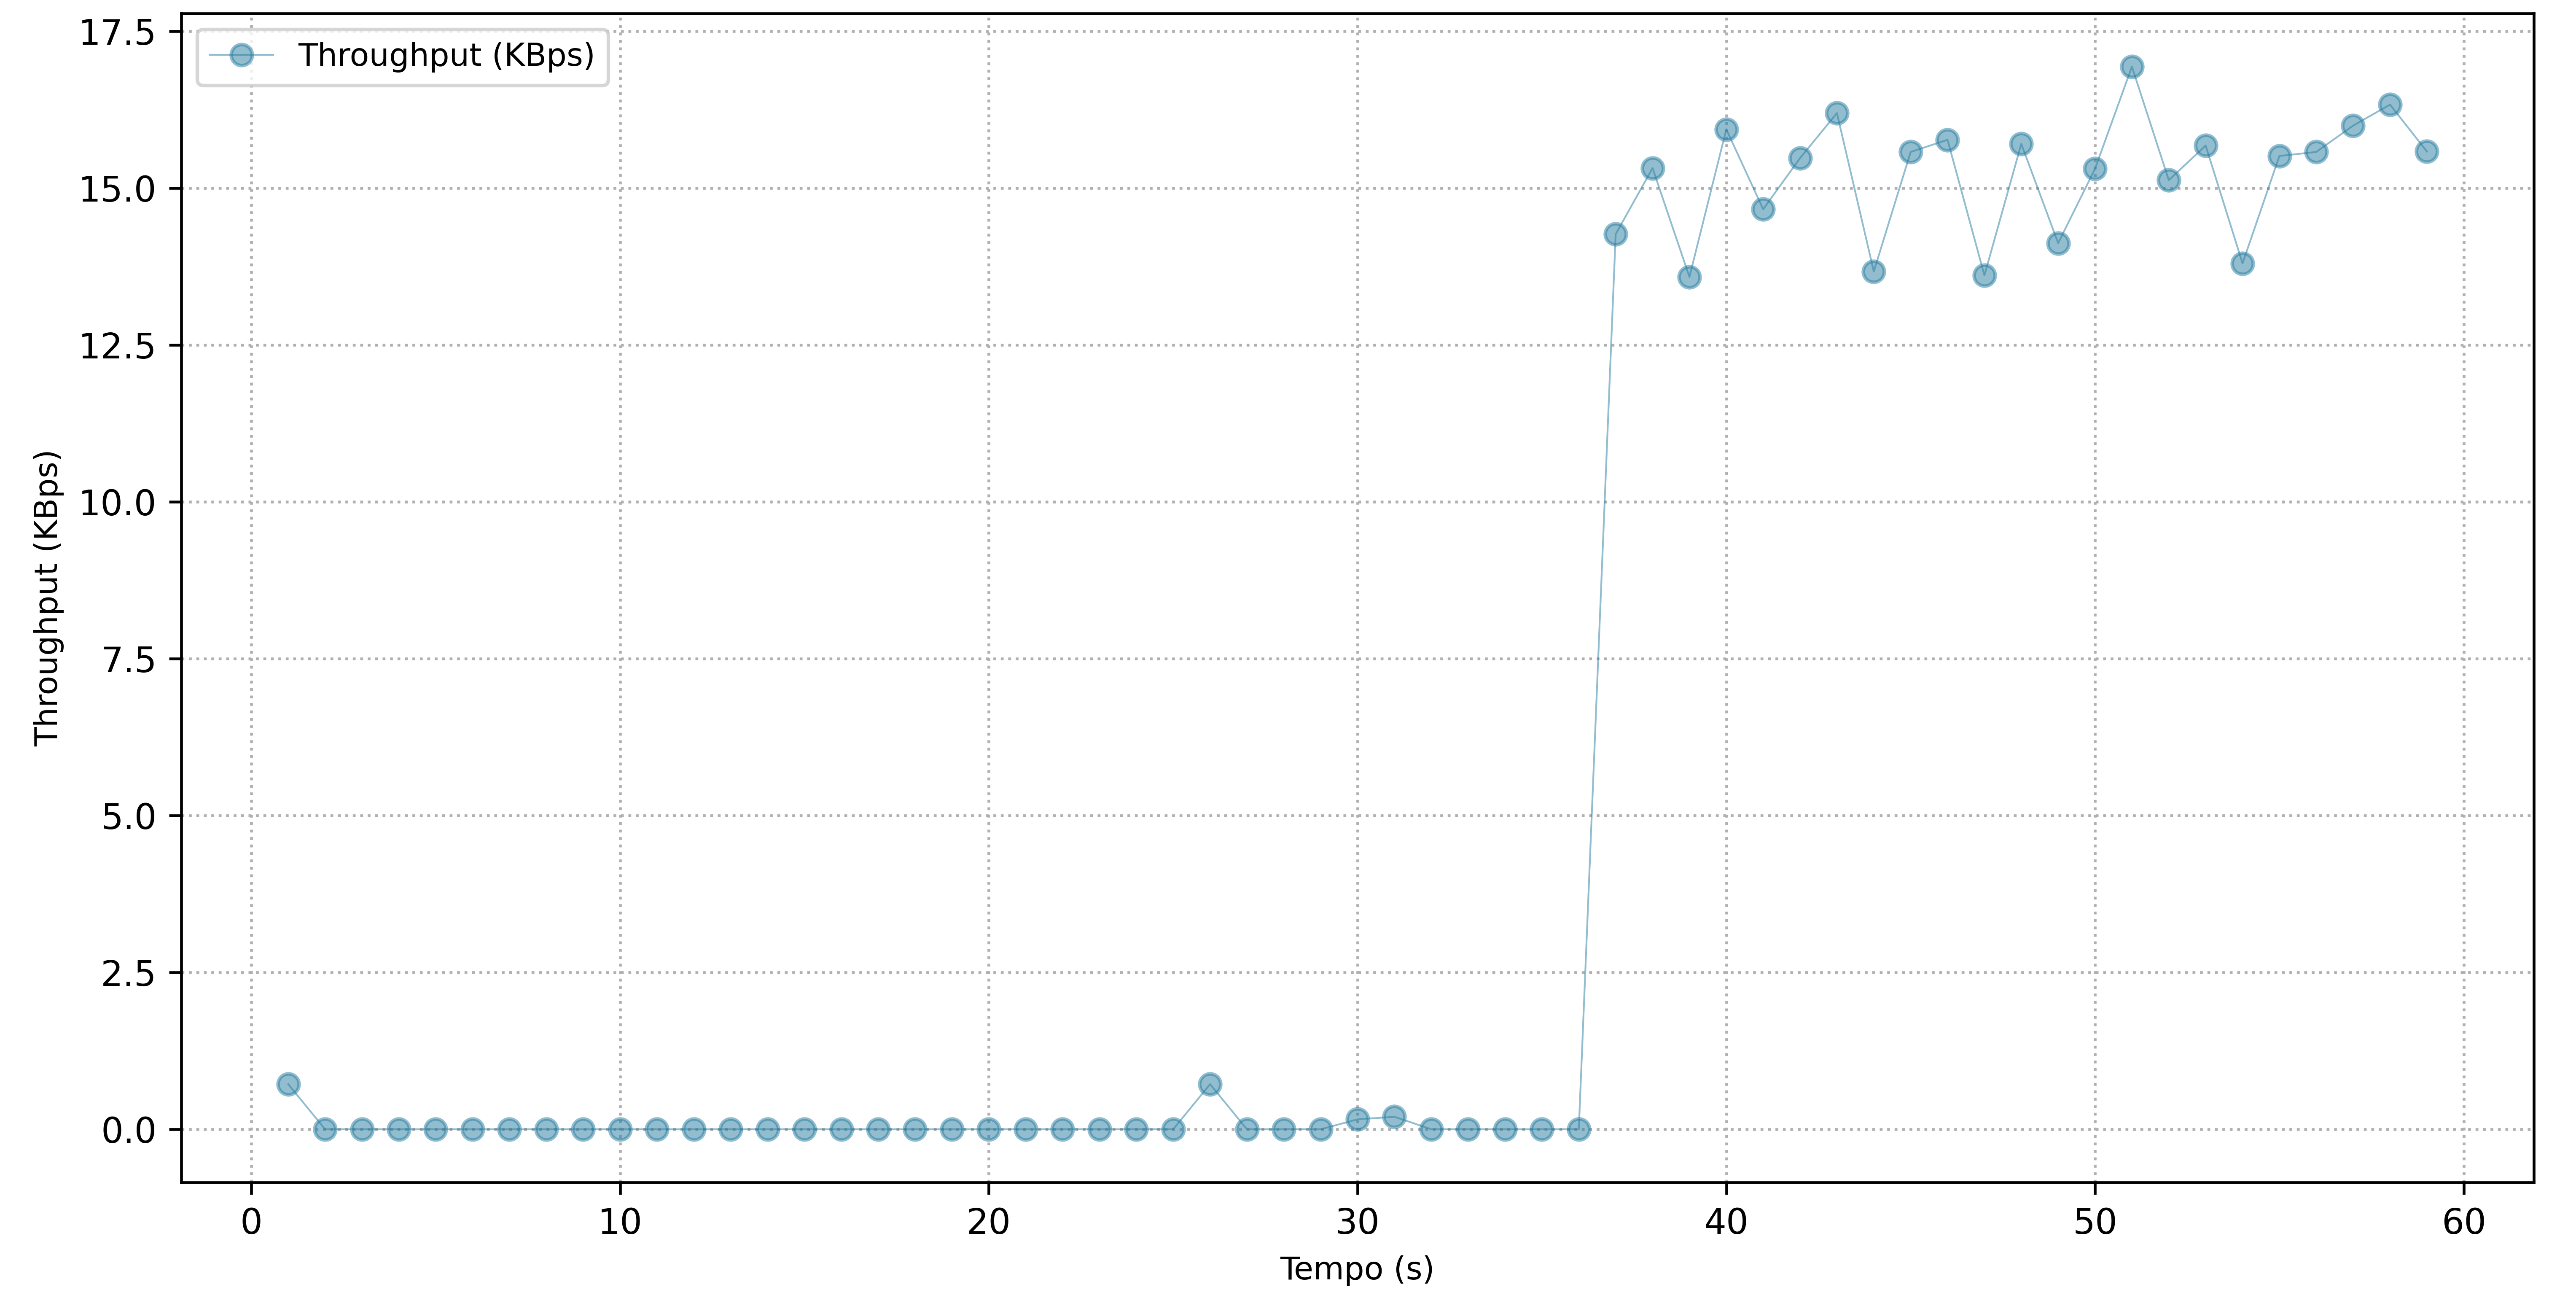
\includegraphics[width=1\textwidth, height=120pt]{USPSC-img/output/cropped/0-normal_local_server-tput.png}
    \end{subfigure}%
    ~ 
    \begin{subfigure}[t]{0.5\textwidth}
        \centering
        \caption{Desempenho}
        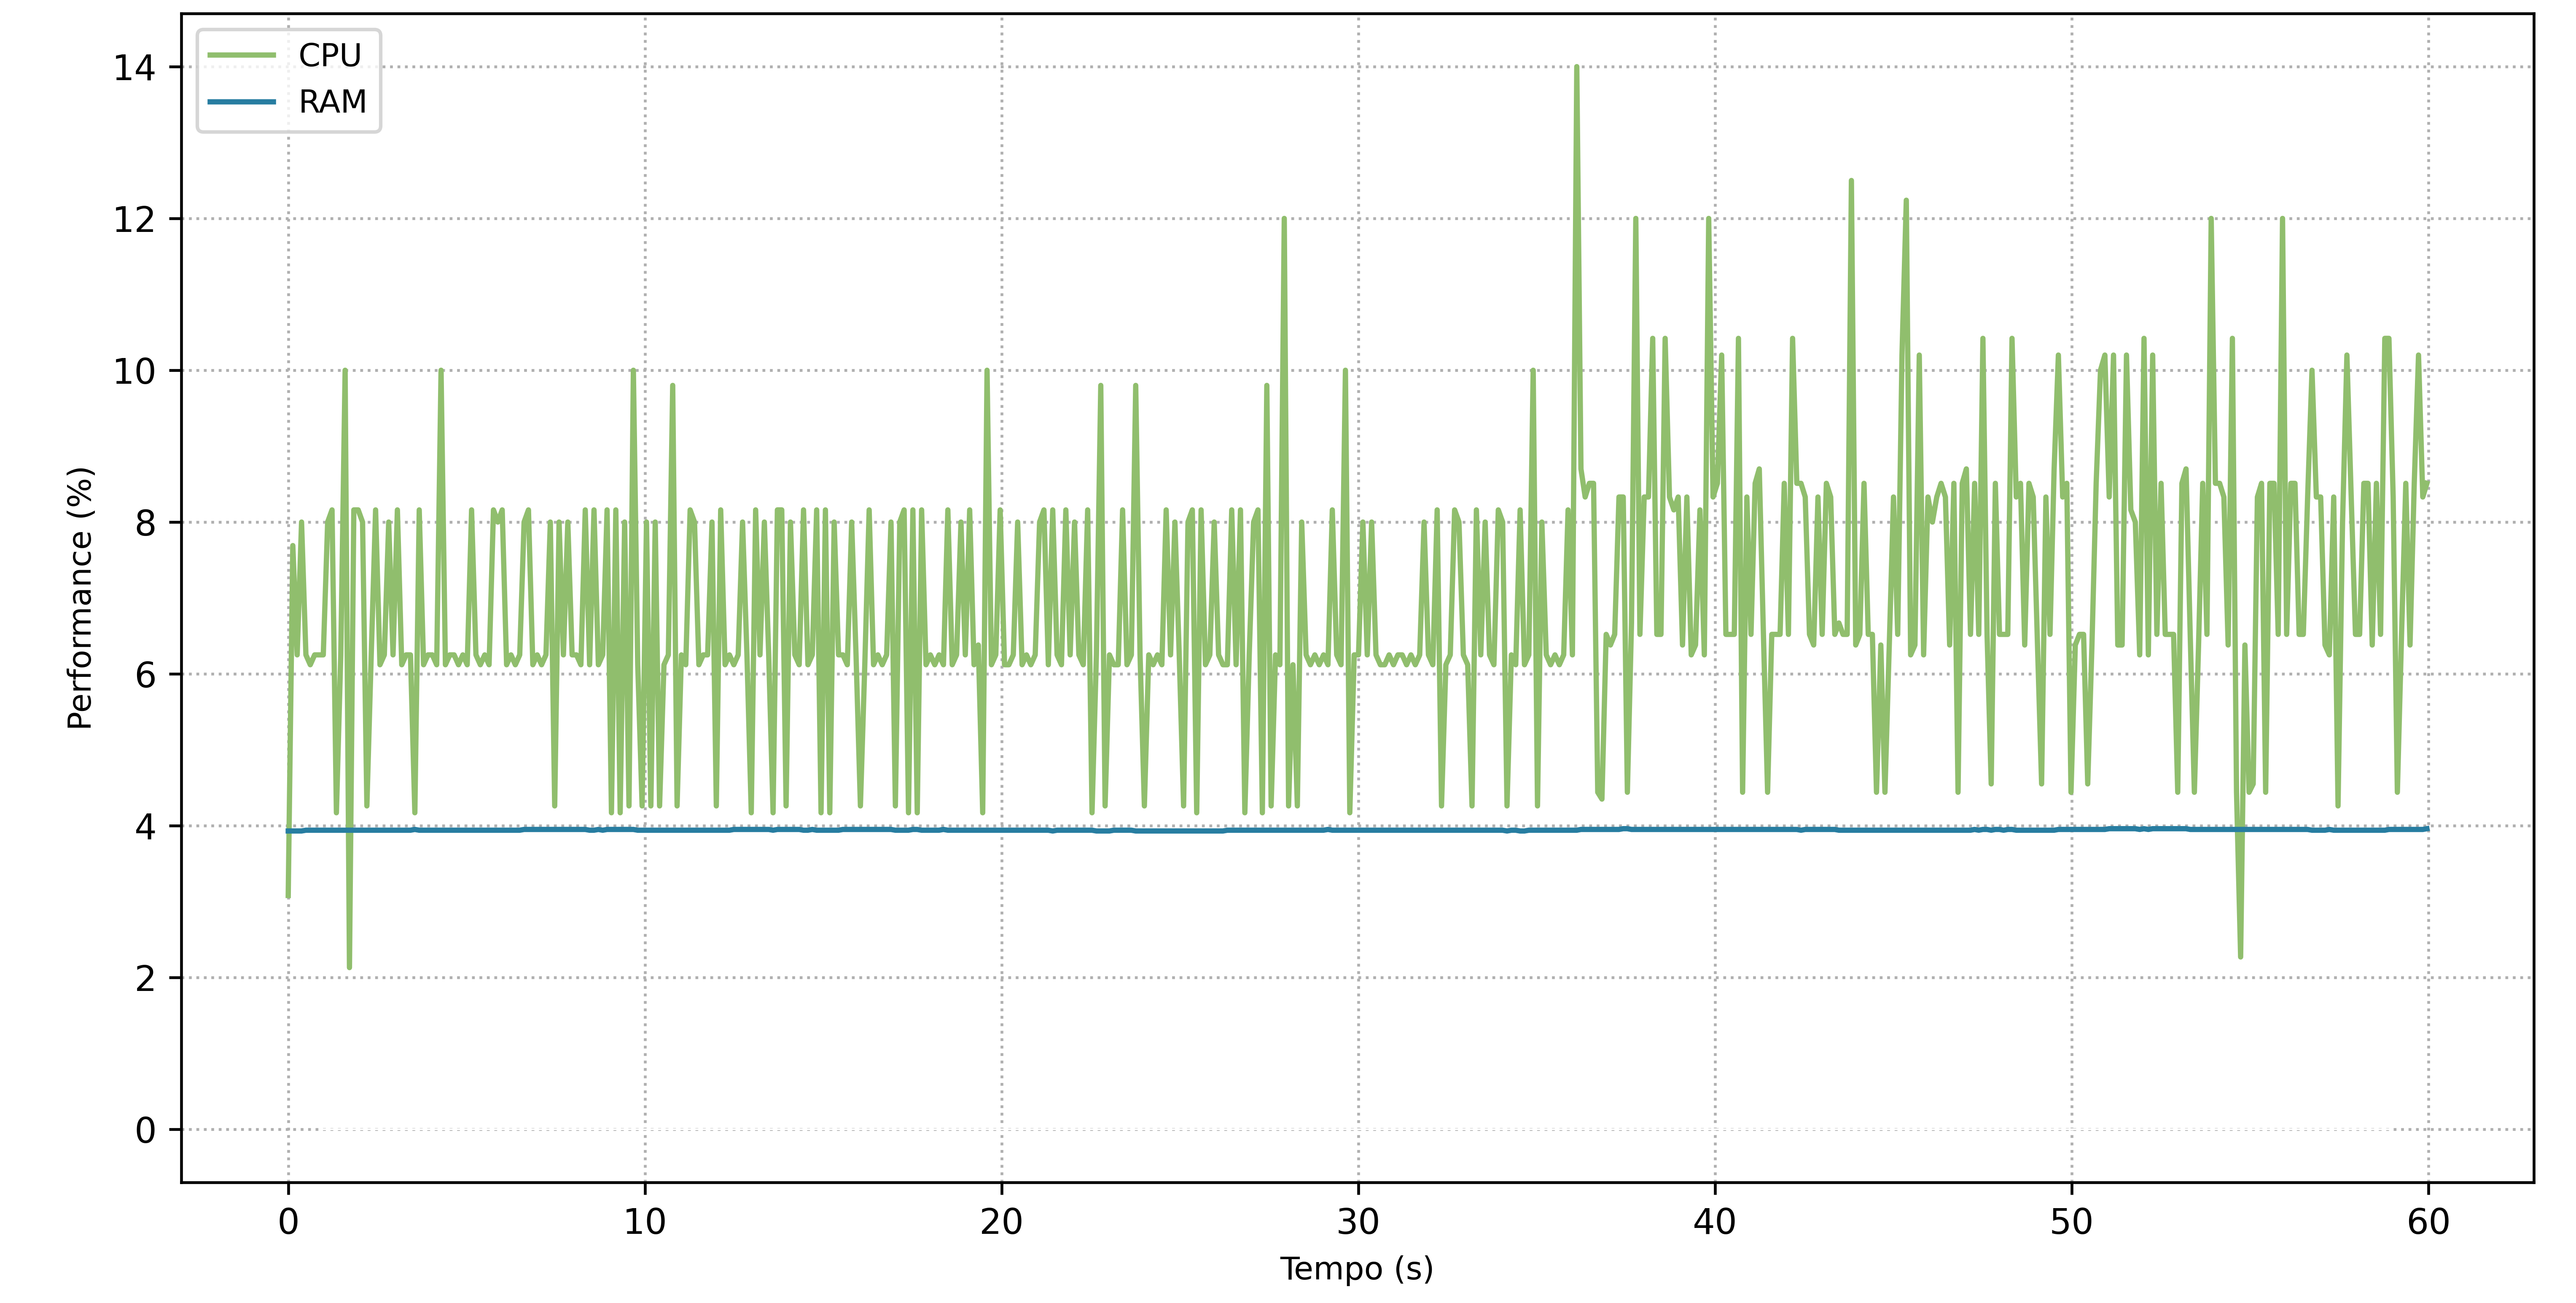
\includegraphics[width=1\textwidth, height=120pt]{USPSC-img/output/cropped/0-normal_local_server-perf.png}
    \end{subfigure}%
    \\
    \begin{subfigure}[t]{0.5\textwidth}
        \centering
        \caption{Pacotes OPC UA}
        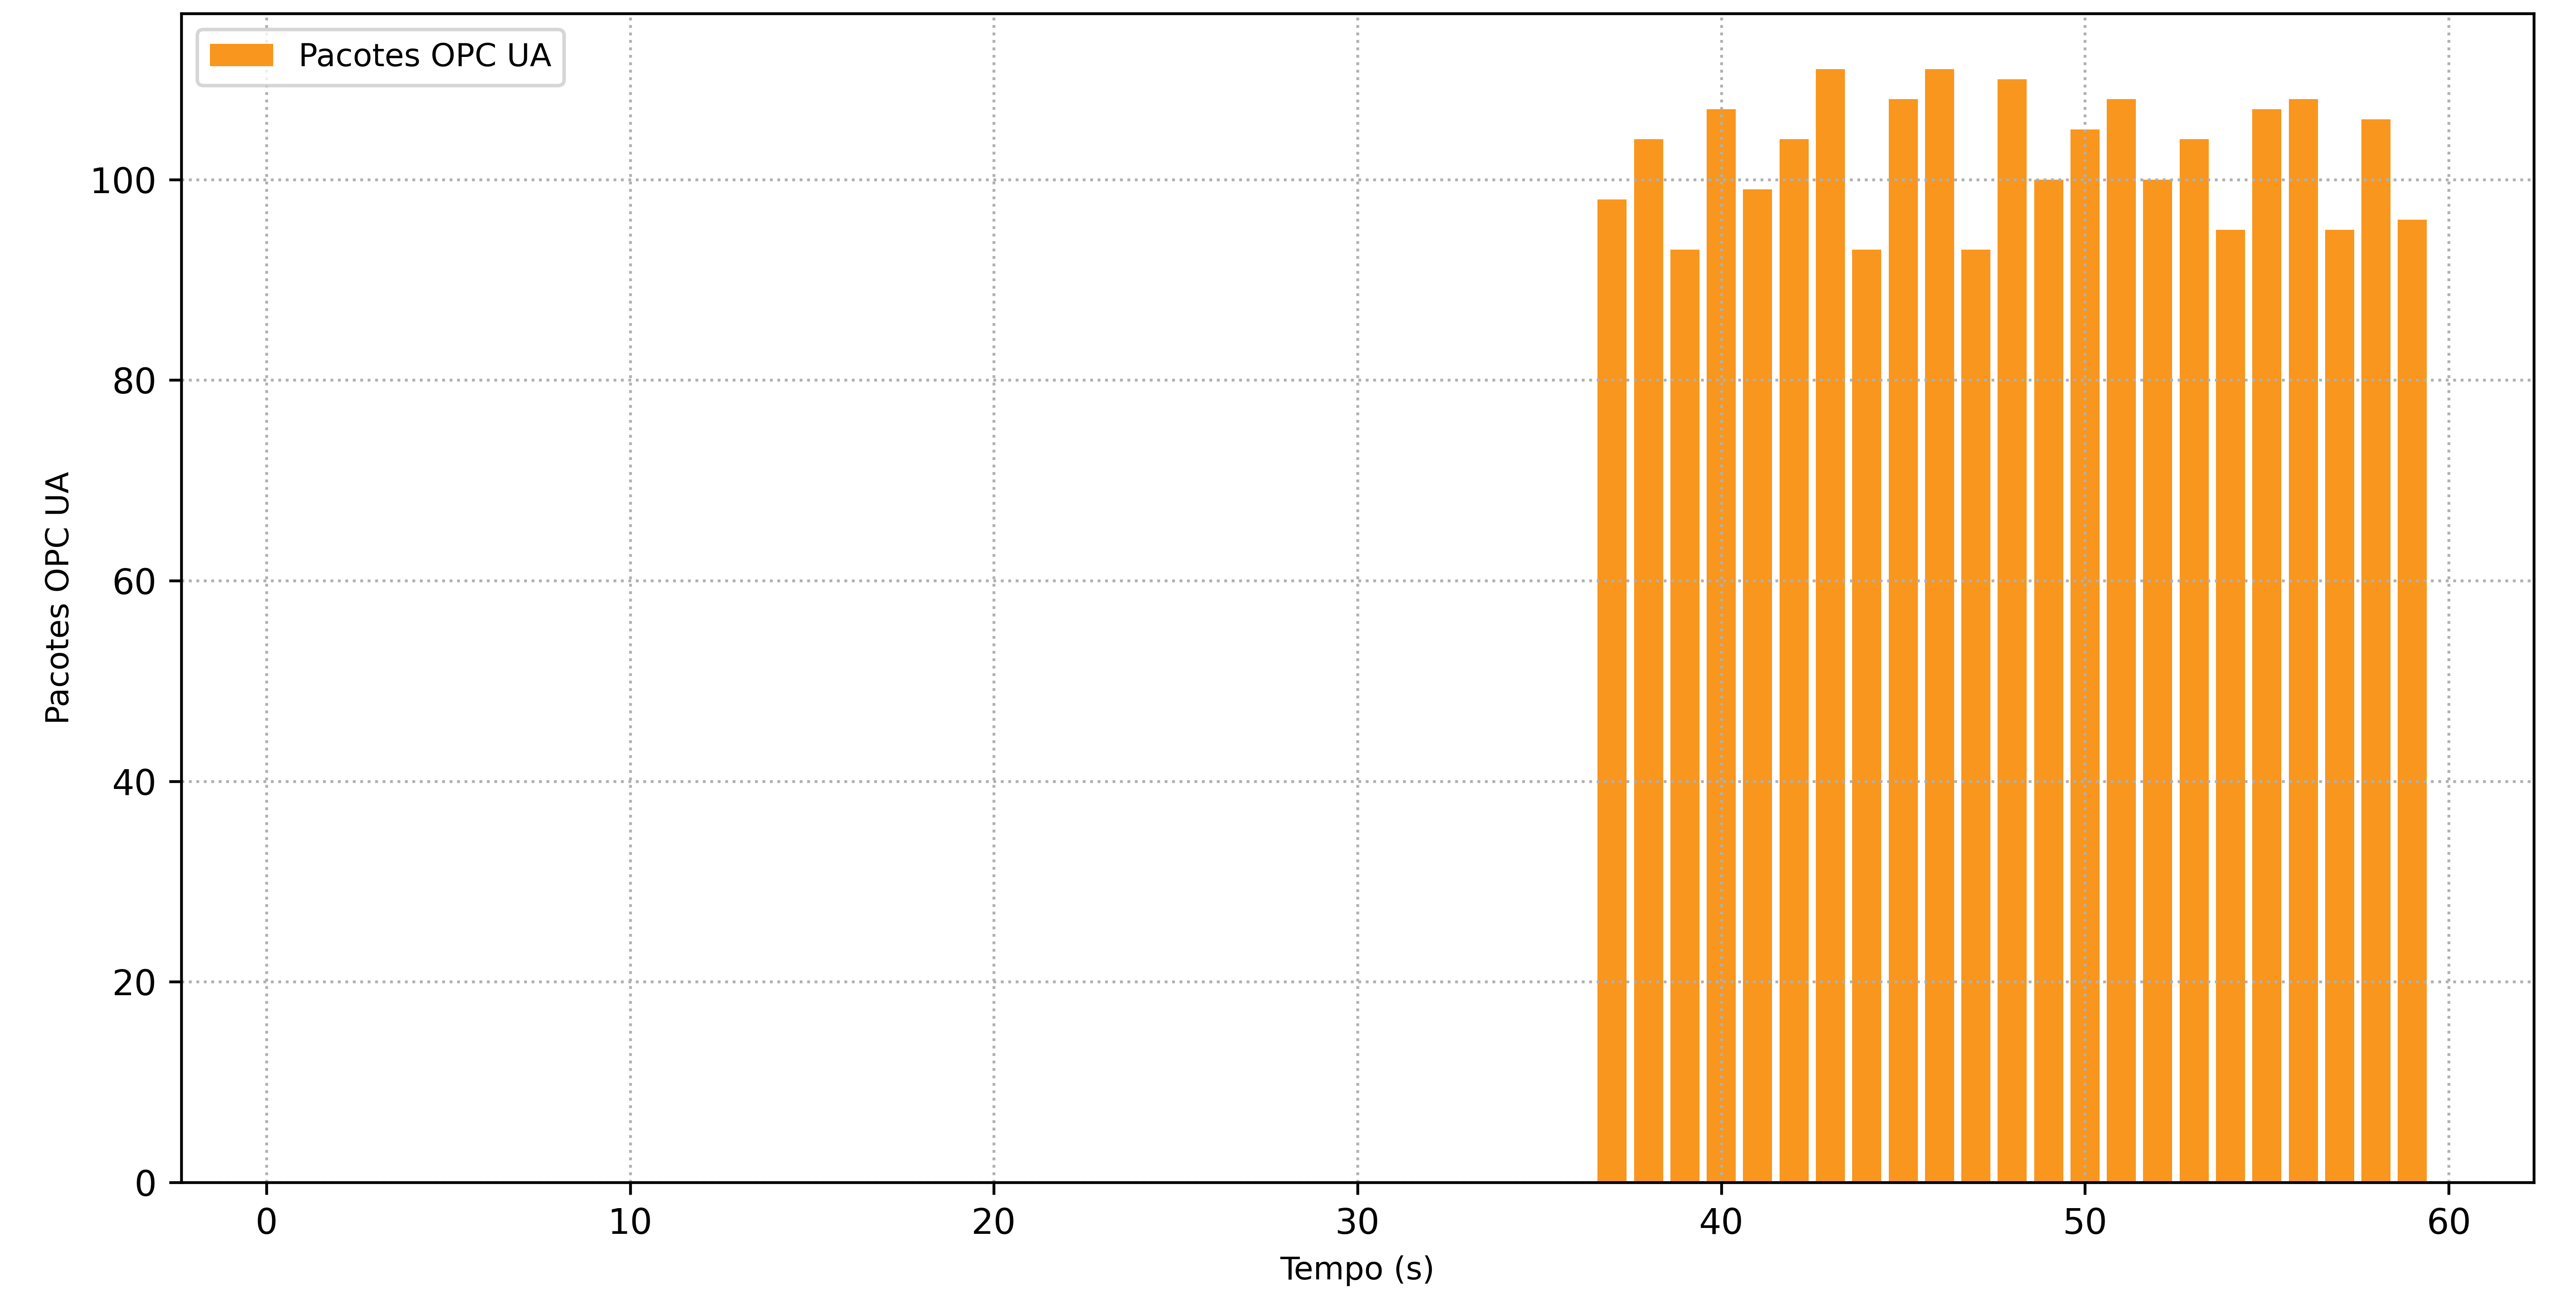
\includegraphics[width=1\textwidth, height=120pt]{USPSC-img/output/cropped/0-normal_local_server-pack.png}
    \end{subfigure}%
    ~
    \begin{subfigure}[t]{0.5\textwidth}
        \centering
        \caption{RTT por pacote}
        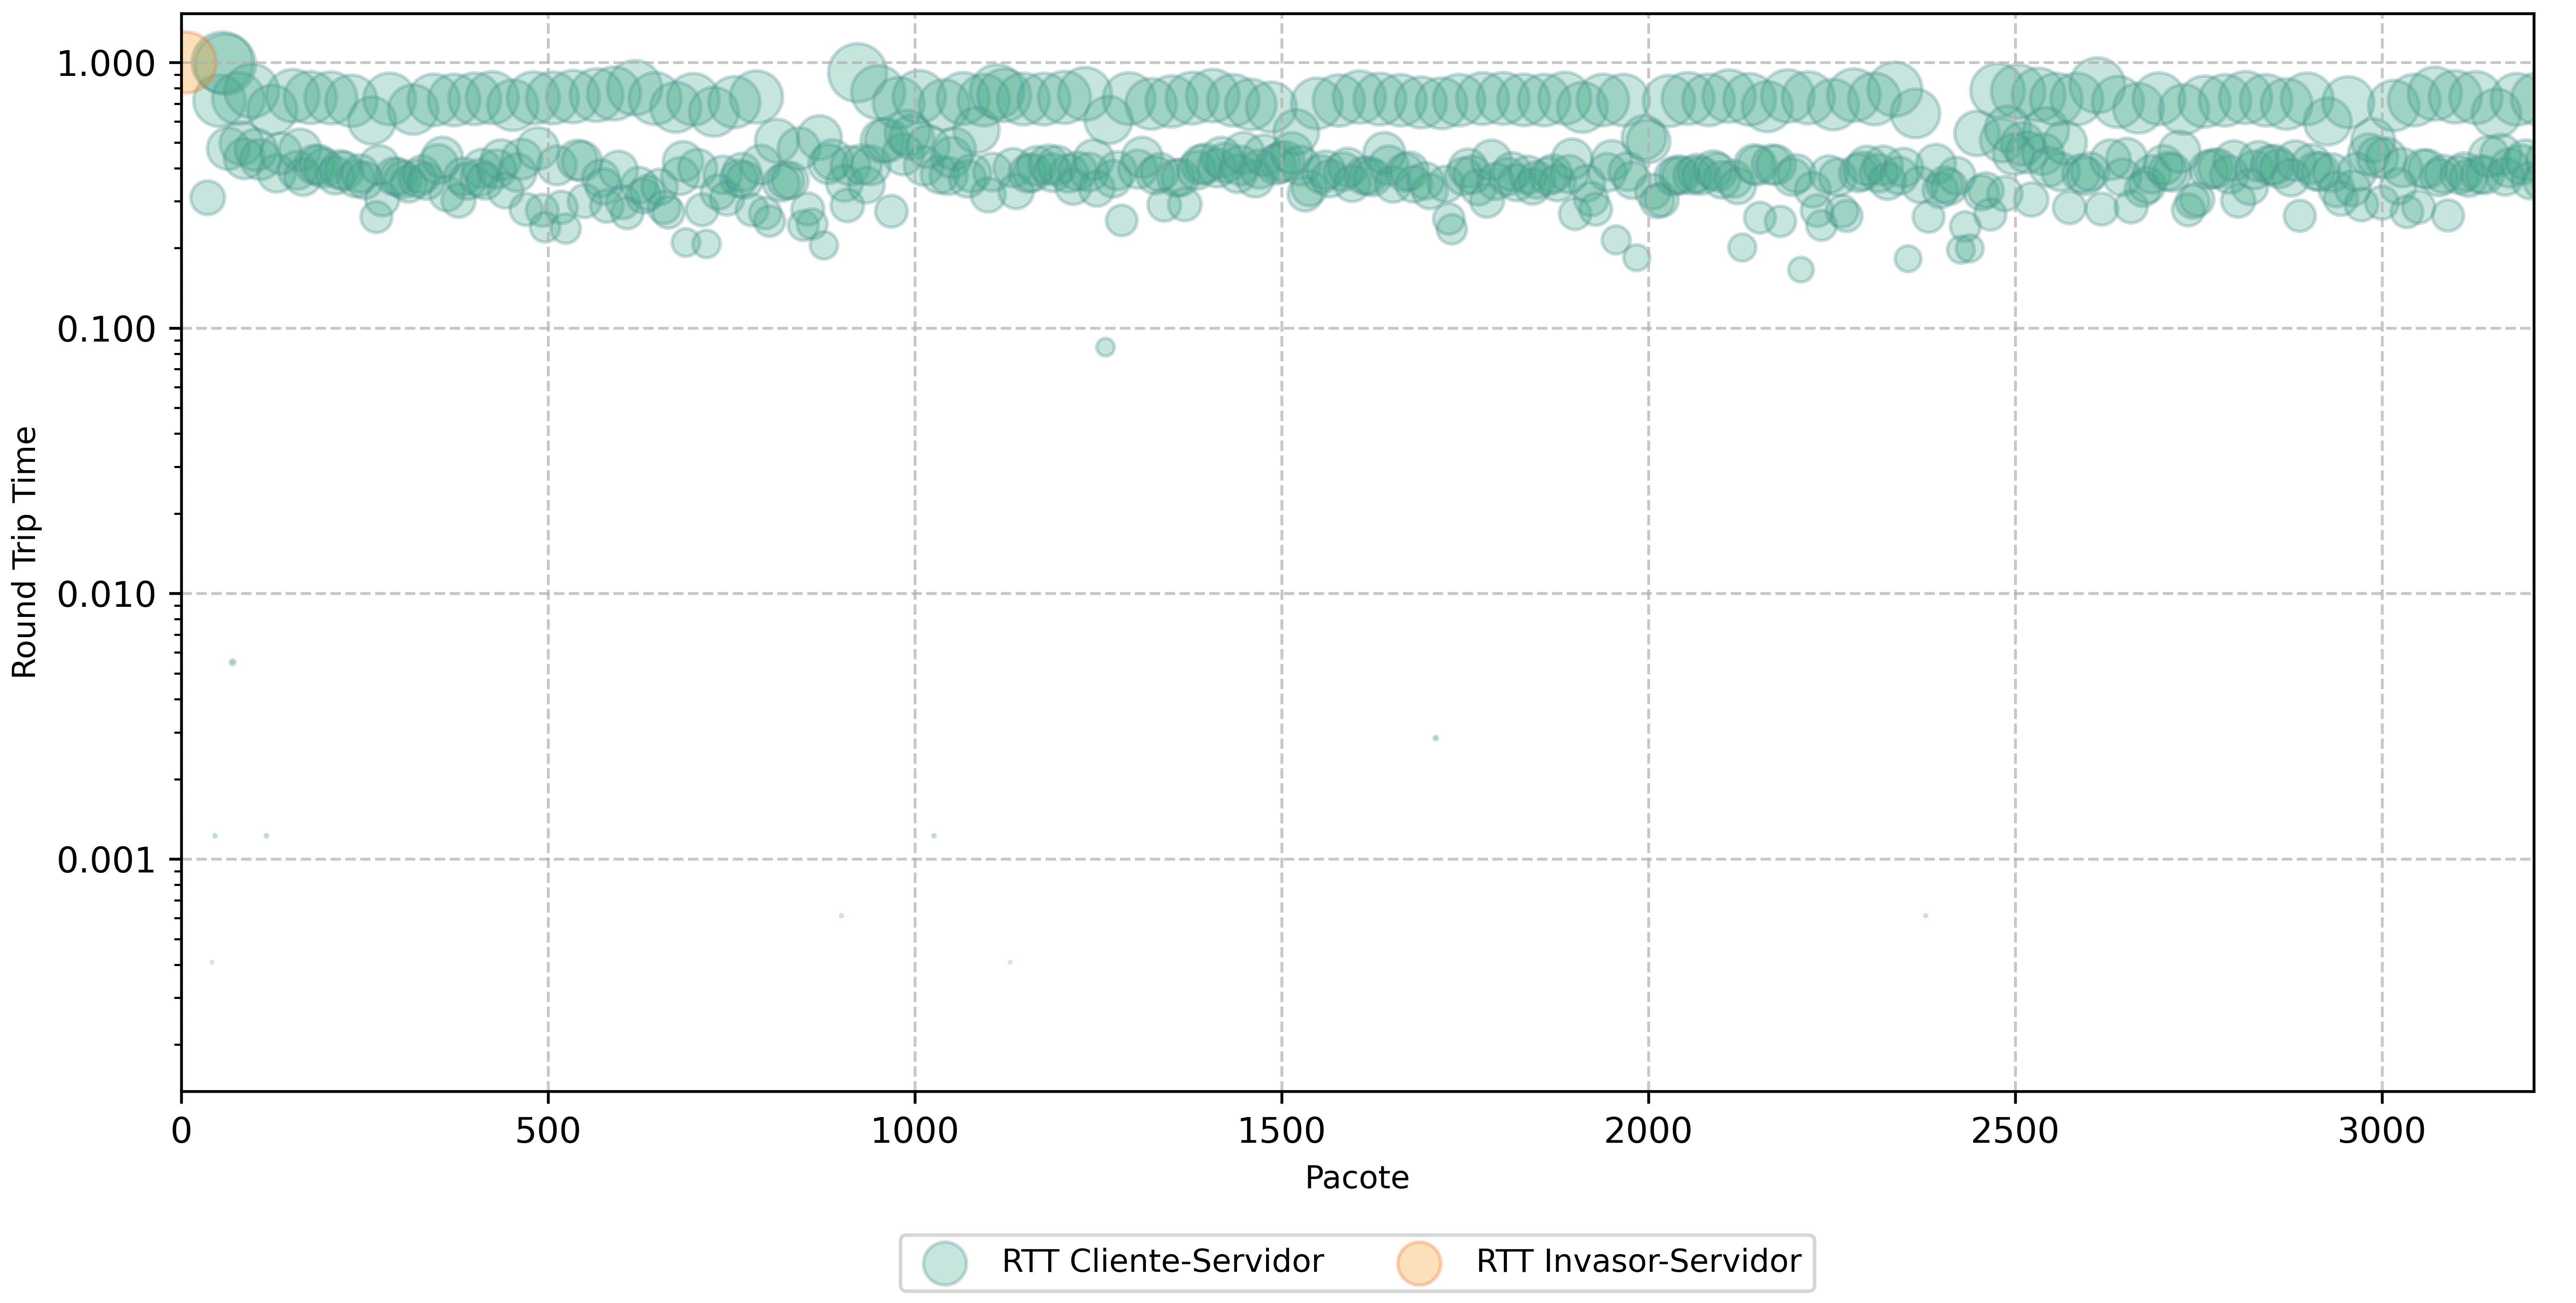
\includegraphics[width=1\textwidth, height=120pt]{USPSC-img/output/cropped/0-normal_local_server-rttp.png}
    \end{subfigure}%
    \legend{Fonte: elaborada pelo autor.}
\end{figure}

Os demais gráficos gerados para os outros cenários podem ser visualizados no \autoref{ap:graficos}.

\section{Análise dos Resultados} \label{sec:analise-resultados}

Nesta seção, são apresentadas as análises dos resultados obtidos a partir dos cenários de ataques cibernéticos executados na bancada experimental. A análise é realizada com base nas métricas de desempenho extraídas dos dados brutos coletados, com o objetivo de avaliar a robustez das redes industriais OPC UA e a variação no desempenho dos componentes ao serem submetidos a tais cenários. Com isso, para organizar melhor as informações, os resultados são divididos em seções que correspondem a cada tipo de ataque

\subsection{\textit{Packet Sniffing}}

Com o auxílio do Wireshark e do Ettercap, este primeiro ataque foi proferido com o objetivo de identificar a presença de vulnerabilidades na rede OPC UA que permitam a interceptação não autorizada de pacotes. Inicialmente, o Ettercap foi empregado para a captura unificada de pacotes, enquanto o Wireshark foi utilizado para a análise detalhada do tráfego de rede. Uma vez que o servidor e o cliente estão conectados, um canal seguro para comunicação é estabelecido. No entanto, o atacante pode explorar vulnerabilidades na rede para interceptar pacotes e obter informações confidenciais, como endereços IP e MAC de todos os dispositivos conectados. No início da captura para o cenário C22, C23 e C24, é possível observar a presença de pacotes de comunicação entre o servidor e o cliente, conforme ilustrado na \autoref{fig:0-sniffing-wireshark}. Note que um filtro foi aplicado para exibir apenas os pacotes de comunicação OPC UA e todos os outros dados foram omitidos nesta visualização. Todo o tráfego relevante relacionado ao protocolo OPC UA apresentado pela \autoref{fig:seqConn} é exposto na análise pelo Wireshark.

\begin{figure}[htbp!]
    \caption{\label{fig:0-sniffing-wireshark}Comunicação interceptada entre o servidor e o cliente OPC UA com modo de segurança `None'}
    \begin{center}
        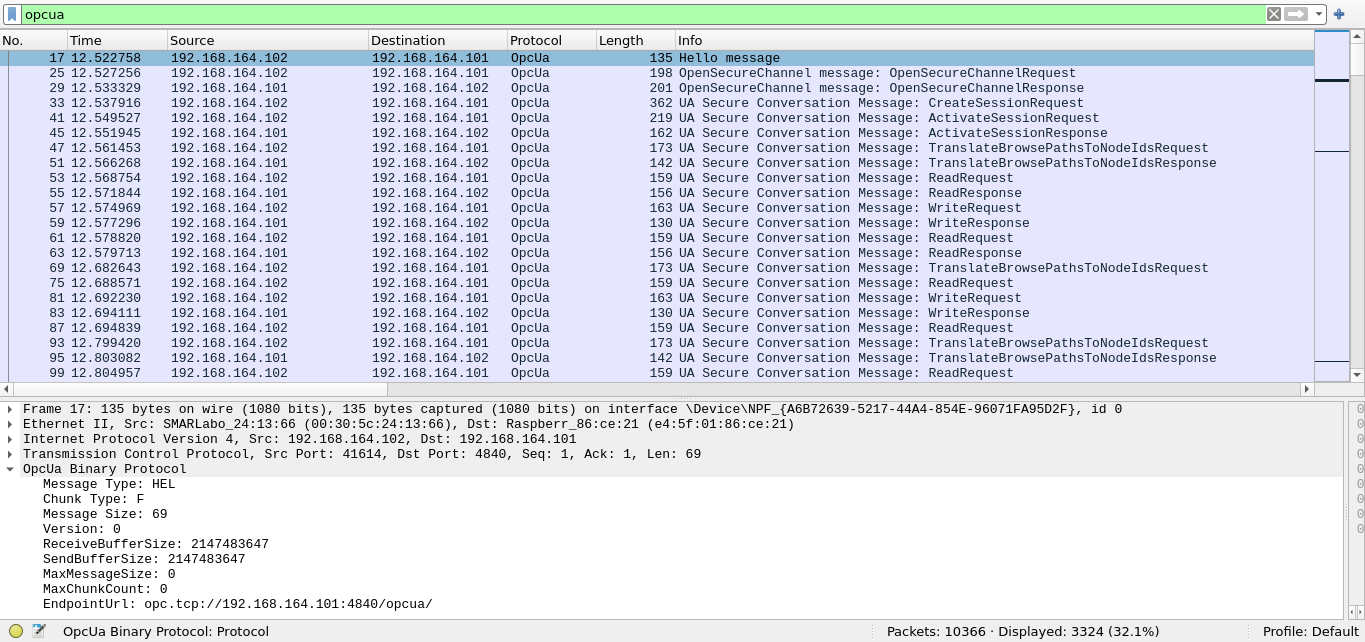
\includegraphics[width=0.972\textwidth]{USPSC-img/0-sniffing-wireshark-filtered-anon.png}
    \end{center}
    \legend{Fonte: elaborada pelo autor.}
\end{figure}

Vale ressaltar que o invasor possui endereço de IP 192.168.164.115, e que está apenas conectado à rede, sem interação física com o servidor (192.168.164.101) ou cliente (192.168.164.102). Para a configuração da comunicação com modo de segurança `None' e `Sign', é possível observar que a capacidade do invasor obter todos os dados sensíveis da comunicação entre o servidor e o cliente, conforme indicado na \autoref{fig:writeRequest}, que representa a coleta do pacote de requisição de escrita (\textit{UA Secure Conversation Message: WriteRequest}) do mesmo valor e nó, do cliente para o servidor.

\begin{figure}[htbp!]
    \centering
    \caption{\label{fig:writeRequest}Informações obtidas pelo invasor com modo de segurança `None' e `Sign'}
    \begin{subfigure}[t]{0.5\textwidth}
        \centering
        \caption{`None'}
        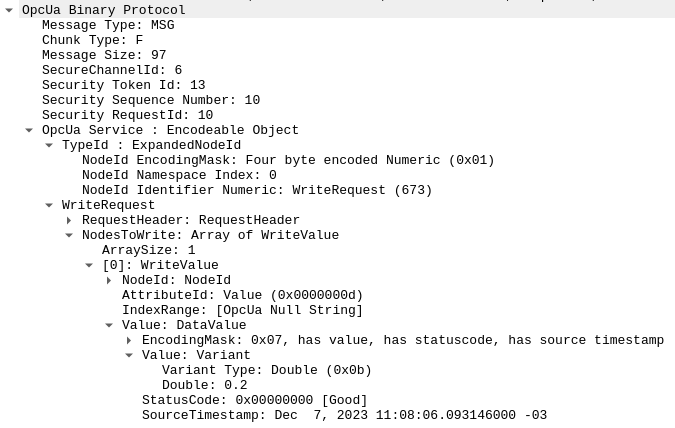
\includegraphics[width=1\textwidth]{USPSC-img/0-sniffing-WriteRequest.png}
    \end{subfigure}%
    ~ 
    \begin{subfigure}[t]{0.5\textwidth}
        \centering
        \caption{`Sign'}
        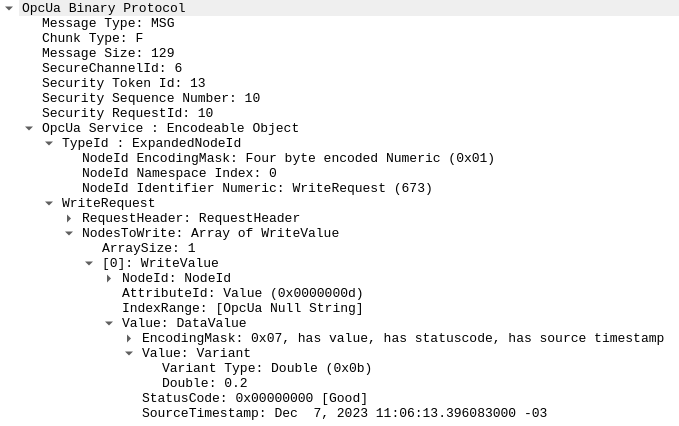
\includegraphics[width=1\textwidth]{USPSC-img/1-sniffing-WriteRequest.png}
    \end{subfigure}%
    \legend{Fonte: elaborada pelo autor.}
\end{figure}

No entanto, ao configurar a comunicação com o modo de segurança `Sign \& Encrypt', o invasor não é capaz de obter informações sensíveis da comunicação entre o servidor e o cliente, pois os dados são, além de assinados, criptografados com políticas de segurança mais robustas, como Basic256Sha256. Assim, para C24, os dados da rede continuam sendo interceptados, mas a comunicação OPC UA não pode ser decifrada, uma vez que todos os pacotes do tipo MSG, com informação \textit{UA Secure Conversation Message: ServiceId [ID]}, possuem o campo de dados \texttt{NodeId EncodingMask} desconhecido.

Portanto, este ataque possui potencial para comprometer a segurança da rede OPC UA ao quebrar a confidencialidade da comunicação, desde que a comunicação seja configurada com modos de segurança mais fracos, como `None' e `Sign'. Tais cenários de ataque evidenciam que, com a utilização de ferramentas simples e acesso ao componente principal da rede, um invasor pode facilmente realizar ataques de captura de pacotes na rede OPC UA, comprometendo dados confidenciais sobre toda a rede. O invasor é capaz de registrar todo o tráfego trocado na rede e, posteriormente, utilizá-lo para outros tipos de ataques, como inserção de pacotes maliciosos (do inglês \textit{packet injection}), DoS, MITM, DDoS, entre outros.

\subsection{\textit{Man in the Middle (MITM)}}

Depois de realizar com sucesso o ataque de \textit{Packet Sniffing}, o invasor terá acesso à uma lista de endereços de todos os dispositivos da rede, além de conhecer informações sensíveis do hospedeiro do servidor OPC UA, incluindo o \texttt{EndpointURI}. Logo, o ataque MITM, pode ser realizado para possibilitar, além da interceptação dos dados, também o controle total da comunicação.

Ambas as técnicas utilizadas para empregar o ataque MITM foram realizadas com sucesso. A execução pela falsificação da tabela ARP, cenários C16, C17 e C18, demonstra que a comunicação é interceptada e redirecionada para o invasor, possibilitando a capturar e modificar os pacotes de dados. A \autoref{fig:0-mitm-wireshark} demonstra a captura de pacotes de comunicação entre o servidor e o cliente, com o invasor atuando como intermediário. Ao comparar com o tráfego apresentado pela \autoref{fig:0-sniffing-wireshark}, é possível observar que o fluxo normal de comunicação é interceptado e redirecionado para o invasor com o endereço MAC \texttt{00:09:5B:A0:5F:F0}.

\begin{figure}[htbp!]
    \centering
    \caption{\label{fig:0-mitm-wireshark}Interceptação de pacotes no ataque MITM com modo de segurança `None'}
    \begin{subfigure}[t]{1\textwidth}
        \centering
        \caption{\texttt{OpenSecureChannelRequest}}
        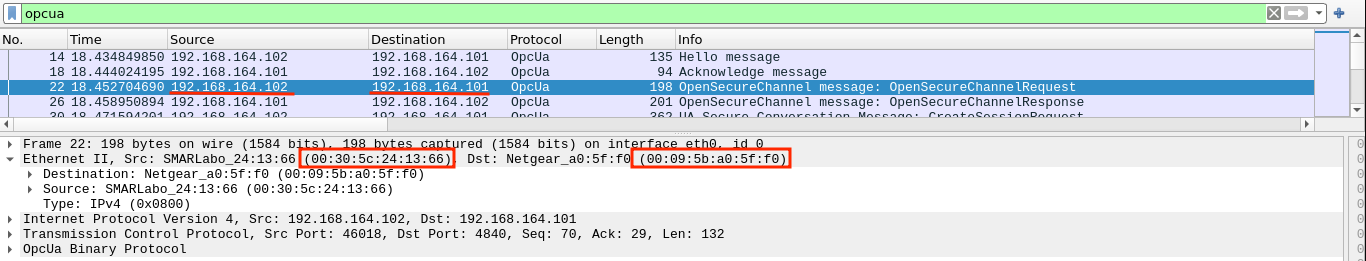
\includegraphics[width=1\textwidth]{USPSC-img/0-mitm-arp_1.png}
    \end{subfigure}%
    \\
    \begin{subfigure}[t]{1\textwidth}
        \centering
        \caption{\texttt{OpenSecureChannelResponse}}
        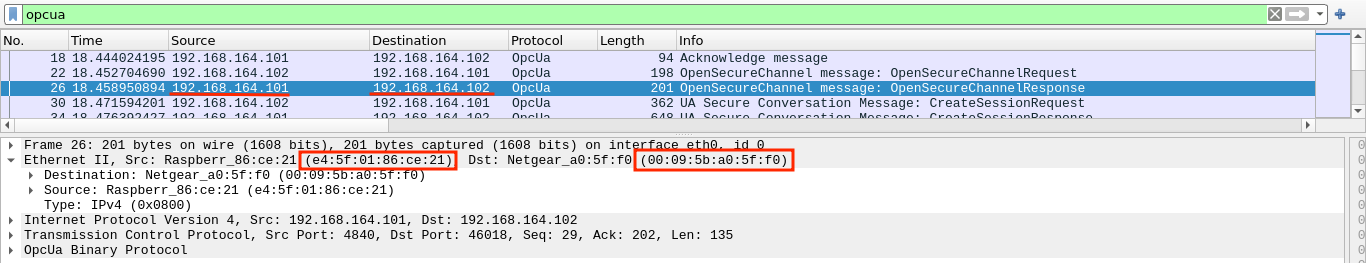
\includegraphics[width=1\textwidth]{USPSC-img/0-mitm-arp_2.png}
    \end{subfigure}%
    \legend{Fonte: elaborada pelo autor.}
\end{figure}

Inicia-se com a etapa de hand-shake entre os agentes, com a saudação do cliente, seguida por um reconhecimento do servidor. Em seguida, o cliente envia uma solicitação \textit{OpenSecureChannelRequest}, à qual o servidor responde com uma \textit{OpenSecureChannelResponse}. Após essa etapa, é criado um \textit{SecureChannel}, e o cliente envia uma \textit{CreateSessionRequest}, que é respondida pelo servidor com uma \textit{CreateSessionResponse}. Uma vez que a sessão é criada, cliente e servidor se ativam usando \textit{ActivateSessionRequest} e \textit{ActivateSessionResponse}. A partir desse ponto, quando o cliente tenta acessar qualquer informação do servidor, observa-se as mensagens \textit{ReadRequest} e \textit{ReadResponse}.

No ataque MITM pelo roubo de portas, cenários C19, C20 e C21, um aumento no \texttt{throughput} é observado, alcançando valores dez vezes maior que o executado pela falsificação da tabela ARP. Essa elevação ocorre devido ao processo de roubo de portas, cuja rede é inundada com pacotes ARP para saturar a tabela ARP do servidor, forçando-o a redirecionar o tráfego para o invasor. Em média, 99.3\% dos pacotes nesses cenários são provenientes do \textit{broadcast} ARP. No entanto, uma vez que esta técnica é empregada com sucesso e a interceptação efetuada, nota-se que a comunicação não é realizada através do invasor, mas sim diretamente entre o servidor e o cliente com a replicação desta para a porta roubada pelo invasor.

A partir de ambas as tecnicas empregadas, nota-se algumas informações confidenciais são obtidas pelo invasor, como o \texttt{EndpointURI} do servidor, o \texttt{SecurityPolicy} e o \texttt{SecurityMode} utilizados na comunicação,  as informações que o servidor OPC UA obtém da rede do chão de fábrica em um ambiente industrial em tempo real. No entanto, vale ressaltar que o invasor não é capaz de decifrar os pacotes de comunicação para o ambiente configurado com o maior nível de segurança (`Sign \& Encrypt') e com políticas de segurança atualizadas. Supõe-se também que para execução deste ataque o invasor tenha acesso físico à rede, o que não deve ser comum em ambientes industriais.

\subsection{\textit{Denial of Service (DoS)}}

Nesta seção, são apresentados os resultados obtidos a partir dos cenários de ataques de negação de serviço (DoS) executados na bancada experimental utilizando cinco técnicas distintas. O objetivo desses ataques é avaliar a capacidade da rede industrial OPC UA de resistir a sobrecargas de tráfego e a variação no desempenho dos componentes ao serem submetidos a tais cenários.

\subsubsection*{\underline{Inundação TCP/IP}}

A execução do ataque pela inundação TCP/IP (cenários C7, C8 e C9) consistiu na varredura inicial da rede para identificar dispositivos e serviços ativos, utilizando Nmap. Os resultados revelaram a presença de um servidor OPC UA em execução e sua respectiva porta aberta para essa comunicação. Isso é suficiente para que o próximo passo seja executado: inundação de pacotes SYN pela comunicação TCP/IP.

Os resultados obtidos para esses cenários indicam que a rede é altamente vulnerável a ataques de inundação TCP/IP, com um aumento significativo no \texttt{throughput} e na taxa de pacotes por segundo. O servidor OPC UA é sobrecarregado com a alta carga de tráfego, resultando em um aumento considerável no uso da CPU e na degradação do desempenho do sistema. O gráfico apresentado na \autoref{fig:perf-dos-tcp} ilustra a variação média no uso da CPU do hospedeiro do servidor OPC UA durante a execução do ataque de inundação TCP/IP. Para facilitar a visualização e análise dos dados, utilizou-se a média móvel para suavizar a série temporal dos dados, atenuando as flutuações de curto prazo e destacando a tendência de longo prazo.

\begin{figure}[htbp!]
    \centering
    \caption{\label{fig:perf-dos-tcp}Variação média no processamento do hospedeiro do servidor OPC UA durante o ataque de inundação TCP/IP}
    \begin{subfigure}[t]{1\textwidth}
        \centering
        \caption{`None'}
        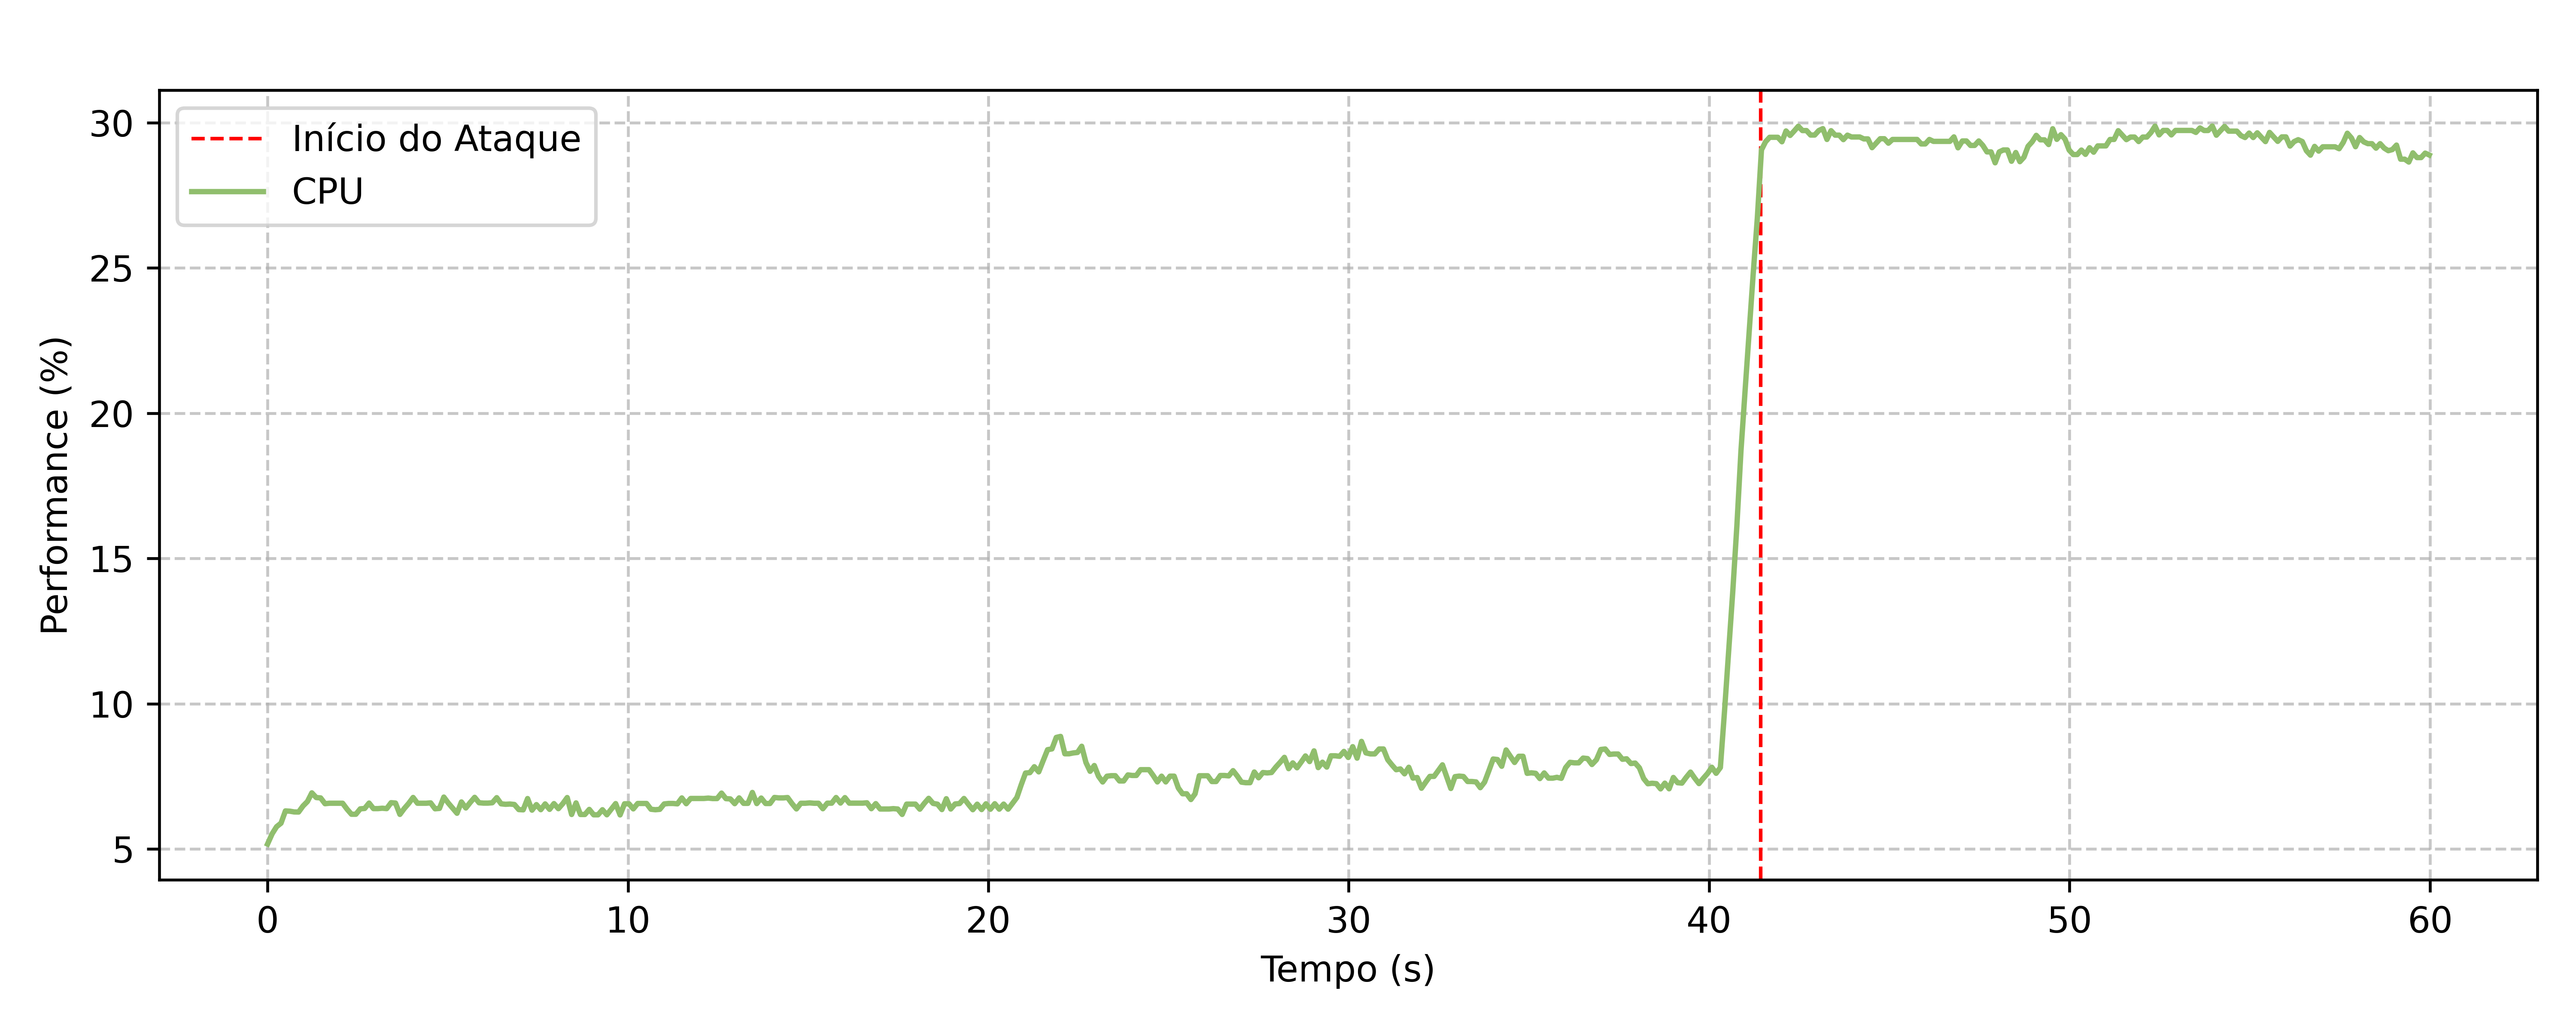
\includegraphics[width=1\textwidth]{USPSC-img/0-dos-hping-cpu.png}
    \end{subfigure}%
    \\
    \begin{subfigure}[t]{1\textwidth}
        \centering
        \caption{`Sign'}
        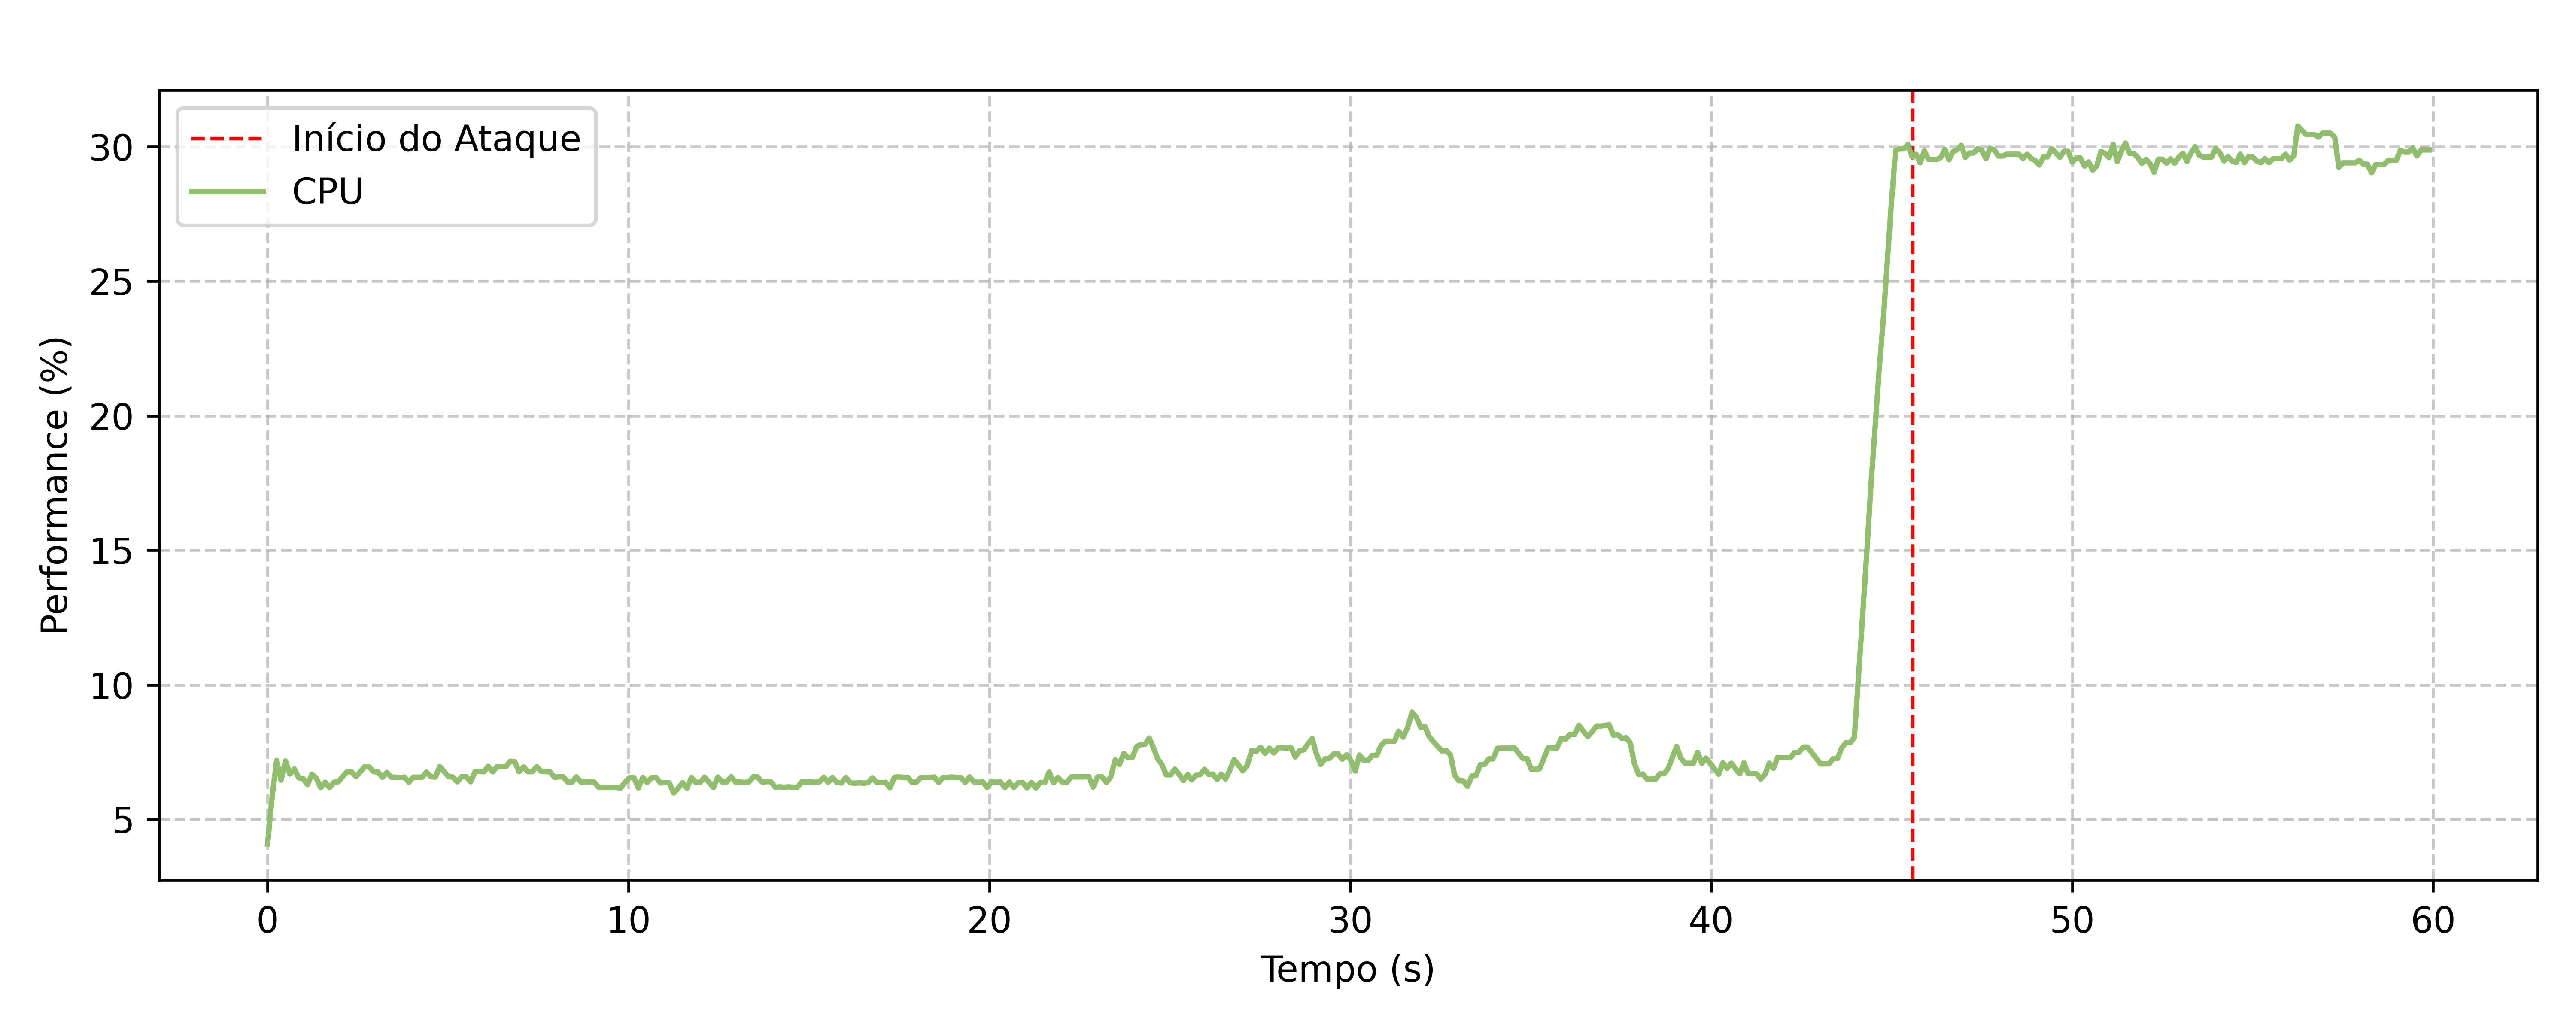
\includegraphics[width=1\textwidth]{USPSC-img/1-dos-hping-cpu.png}
    \end{subfigure}%
    \\
    \begin{subfigure}[t]{1\textwidth}
        \centering
        \caption{`Sign \& Encrypt'}
        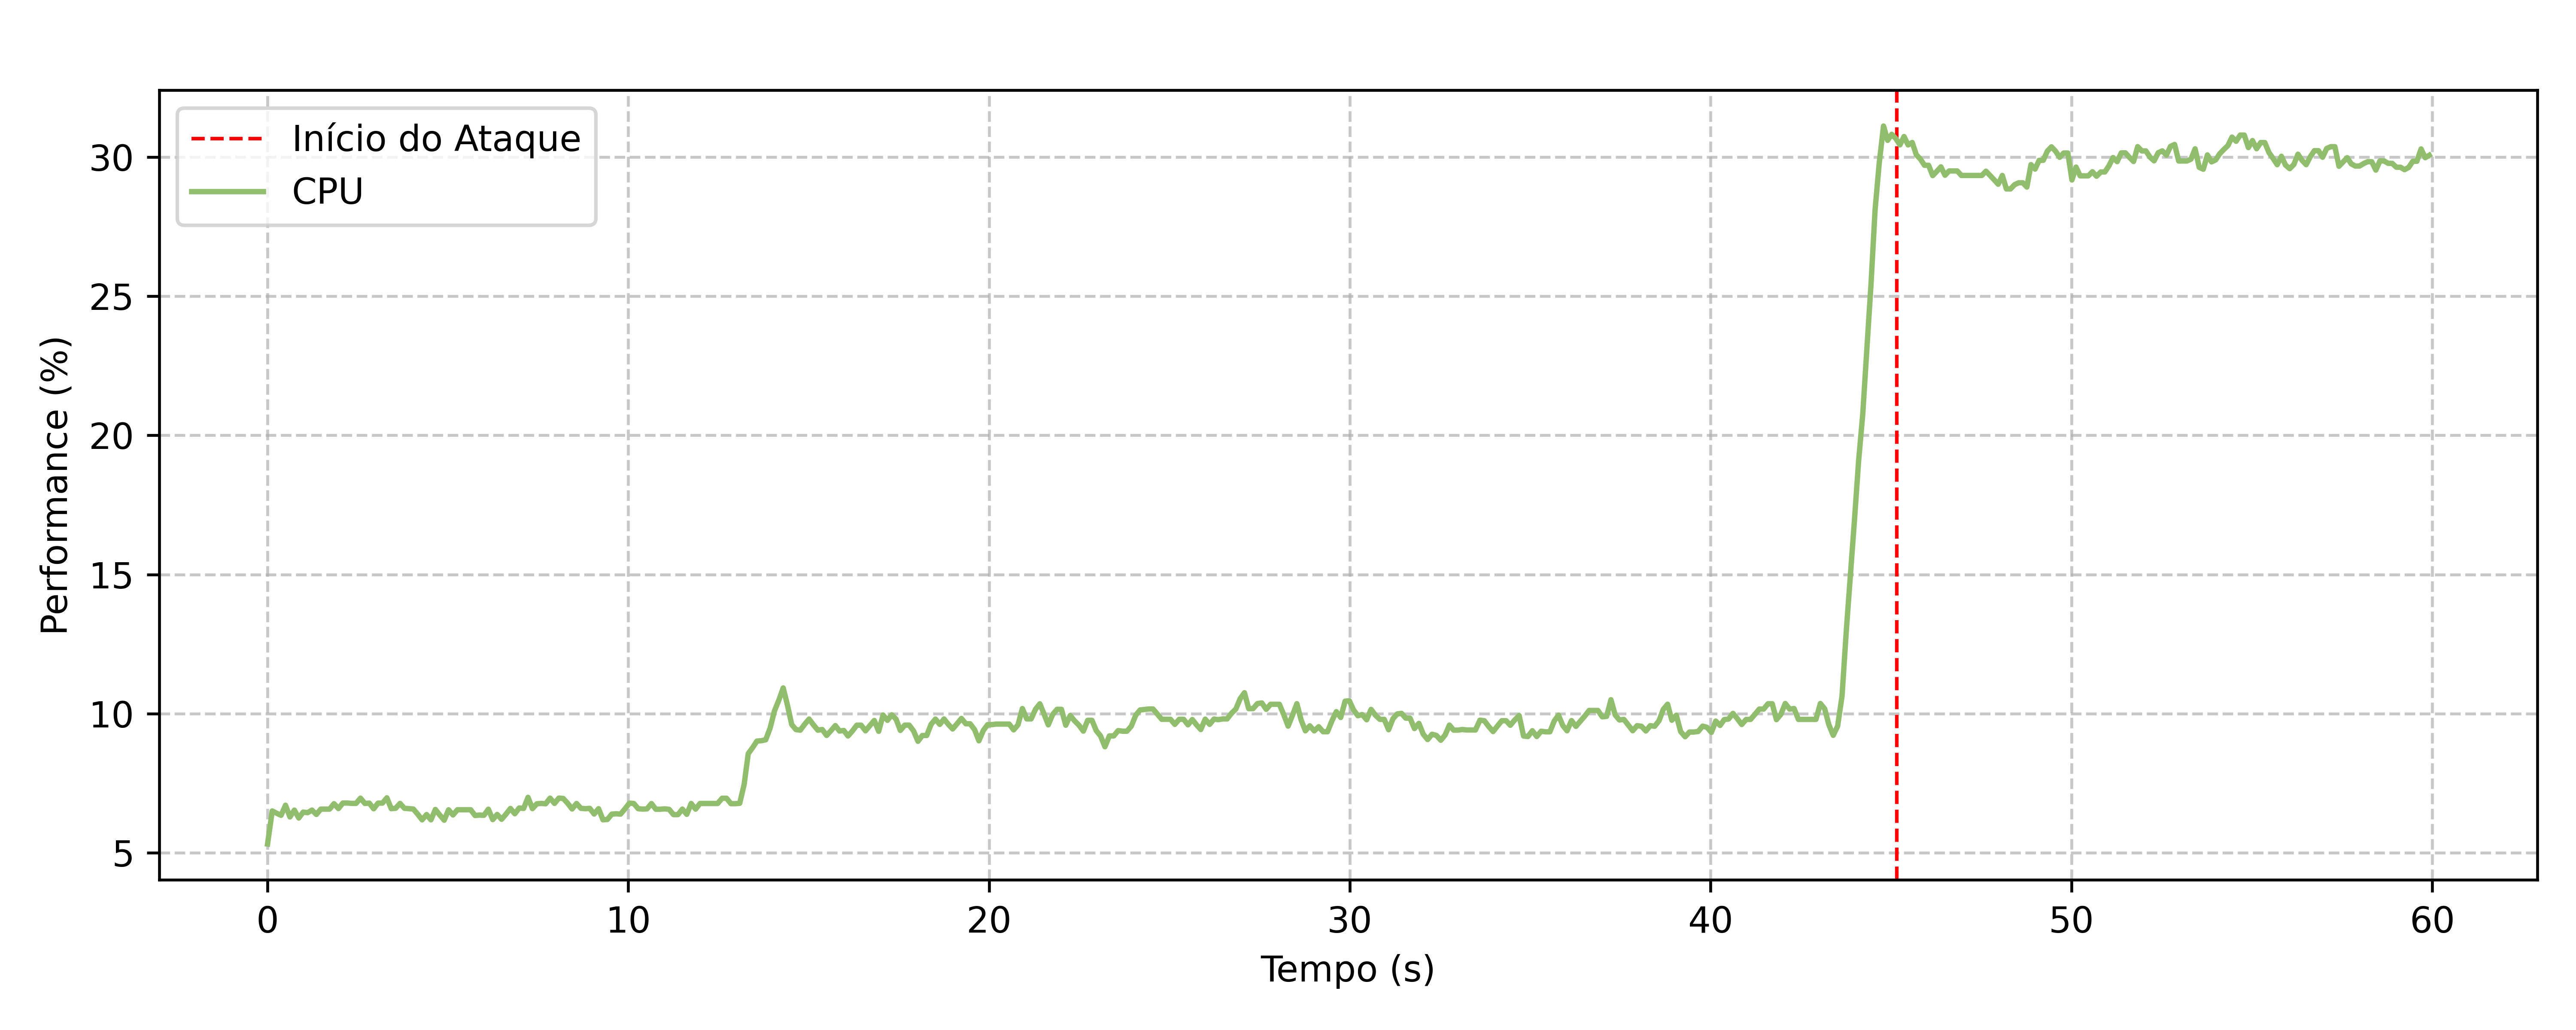
\includegraphics[width=1\textwidth]{USPSC-img/2-dos-hping-cpu.png}
    \end{subfigure}%
    \legend{Fonte: elaborada pelo autor.}
\end{figure}

Em média, o aumento de 275\% no processamento ao início do ataque para qualquer cenário de configuração de segurança, indica que o servidor OPC UA é altamente vulnerável a ataques de inundação TCP/IP, visto que os ataques foram executados em um ambiente controlado e nenhuma outra tarefa estava sendo processada pelo controlador. A alta carga de tráfego gerada por esse tipo de ataque pode levar à degradação do serviço, à interrupção da comunicação e à perda de dados críticos. Portanto, é essencial implementar medidas de segurança robustas para proteger a rede contra esse tipo de ataque e garantir a disponibilidade e a integridade dos sistemas industriais.

No entanto, vale ressaltar que este ataque não foi direcionado para o protocolo OPC UA, mas sim para a camada de transporte (quarta camada do modelo OSI). Portanto, embora a comunicação OPC UA não seja afetada diretamente, o corrompimento da infraestrutura de rede subjacente pode apresentar impactos significativos na comunicação OPC UA, especialmente em ambientes industriais, cuja a disponibilidade e a integridade dos sistemas são críticas.

\subsubsection*{\underline{Loop infinito na cadeia de certificados}}

A tecnologia OPC UA demonstrou uma resistência considerável ao ataque de negação de serviço pelo loop infinito na cadeia de certificados. Essa análise pode ser realizada com base nos gráficos de RTT da comunicação. A Figura \ref{fig:0-dos-cert-rttp} apresenta a variação média do RTT normalizado por pacote durante a execução do ataque para o cenário C3.

\begin{figure}[htbp!]
    \caption{\label{fig:0-dos-cert-rttp}Tempo de resposta normalizado por pacote durante o ataque de loop infinito na cadeia de certificados - nível de segurança: `Sign \& Encrypt'}
    \begin{center}
        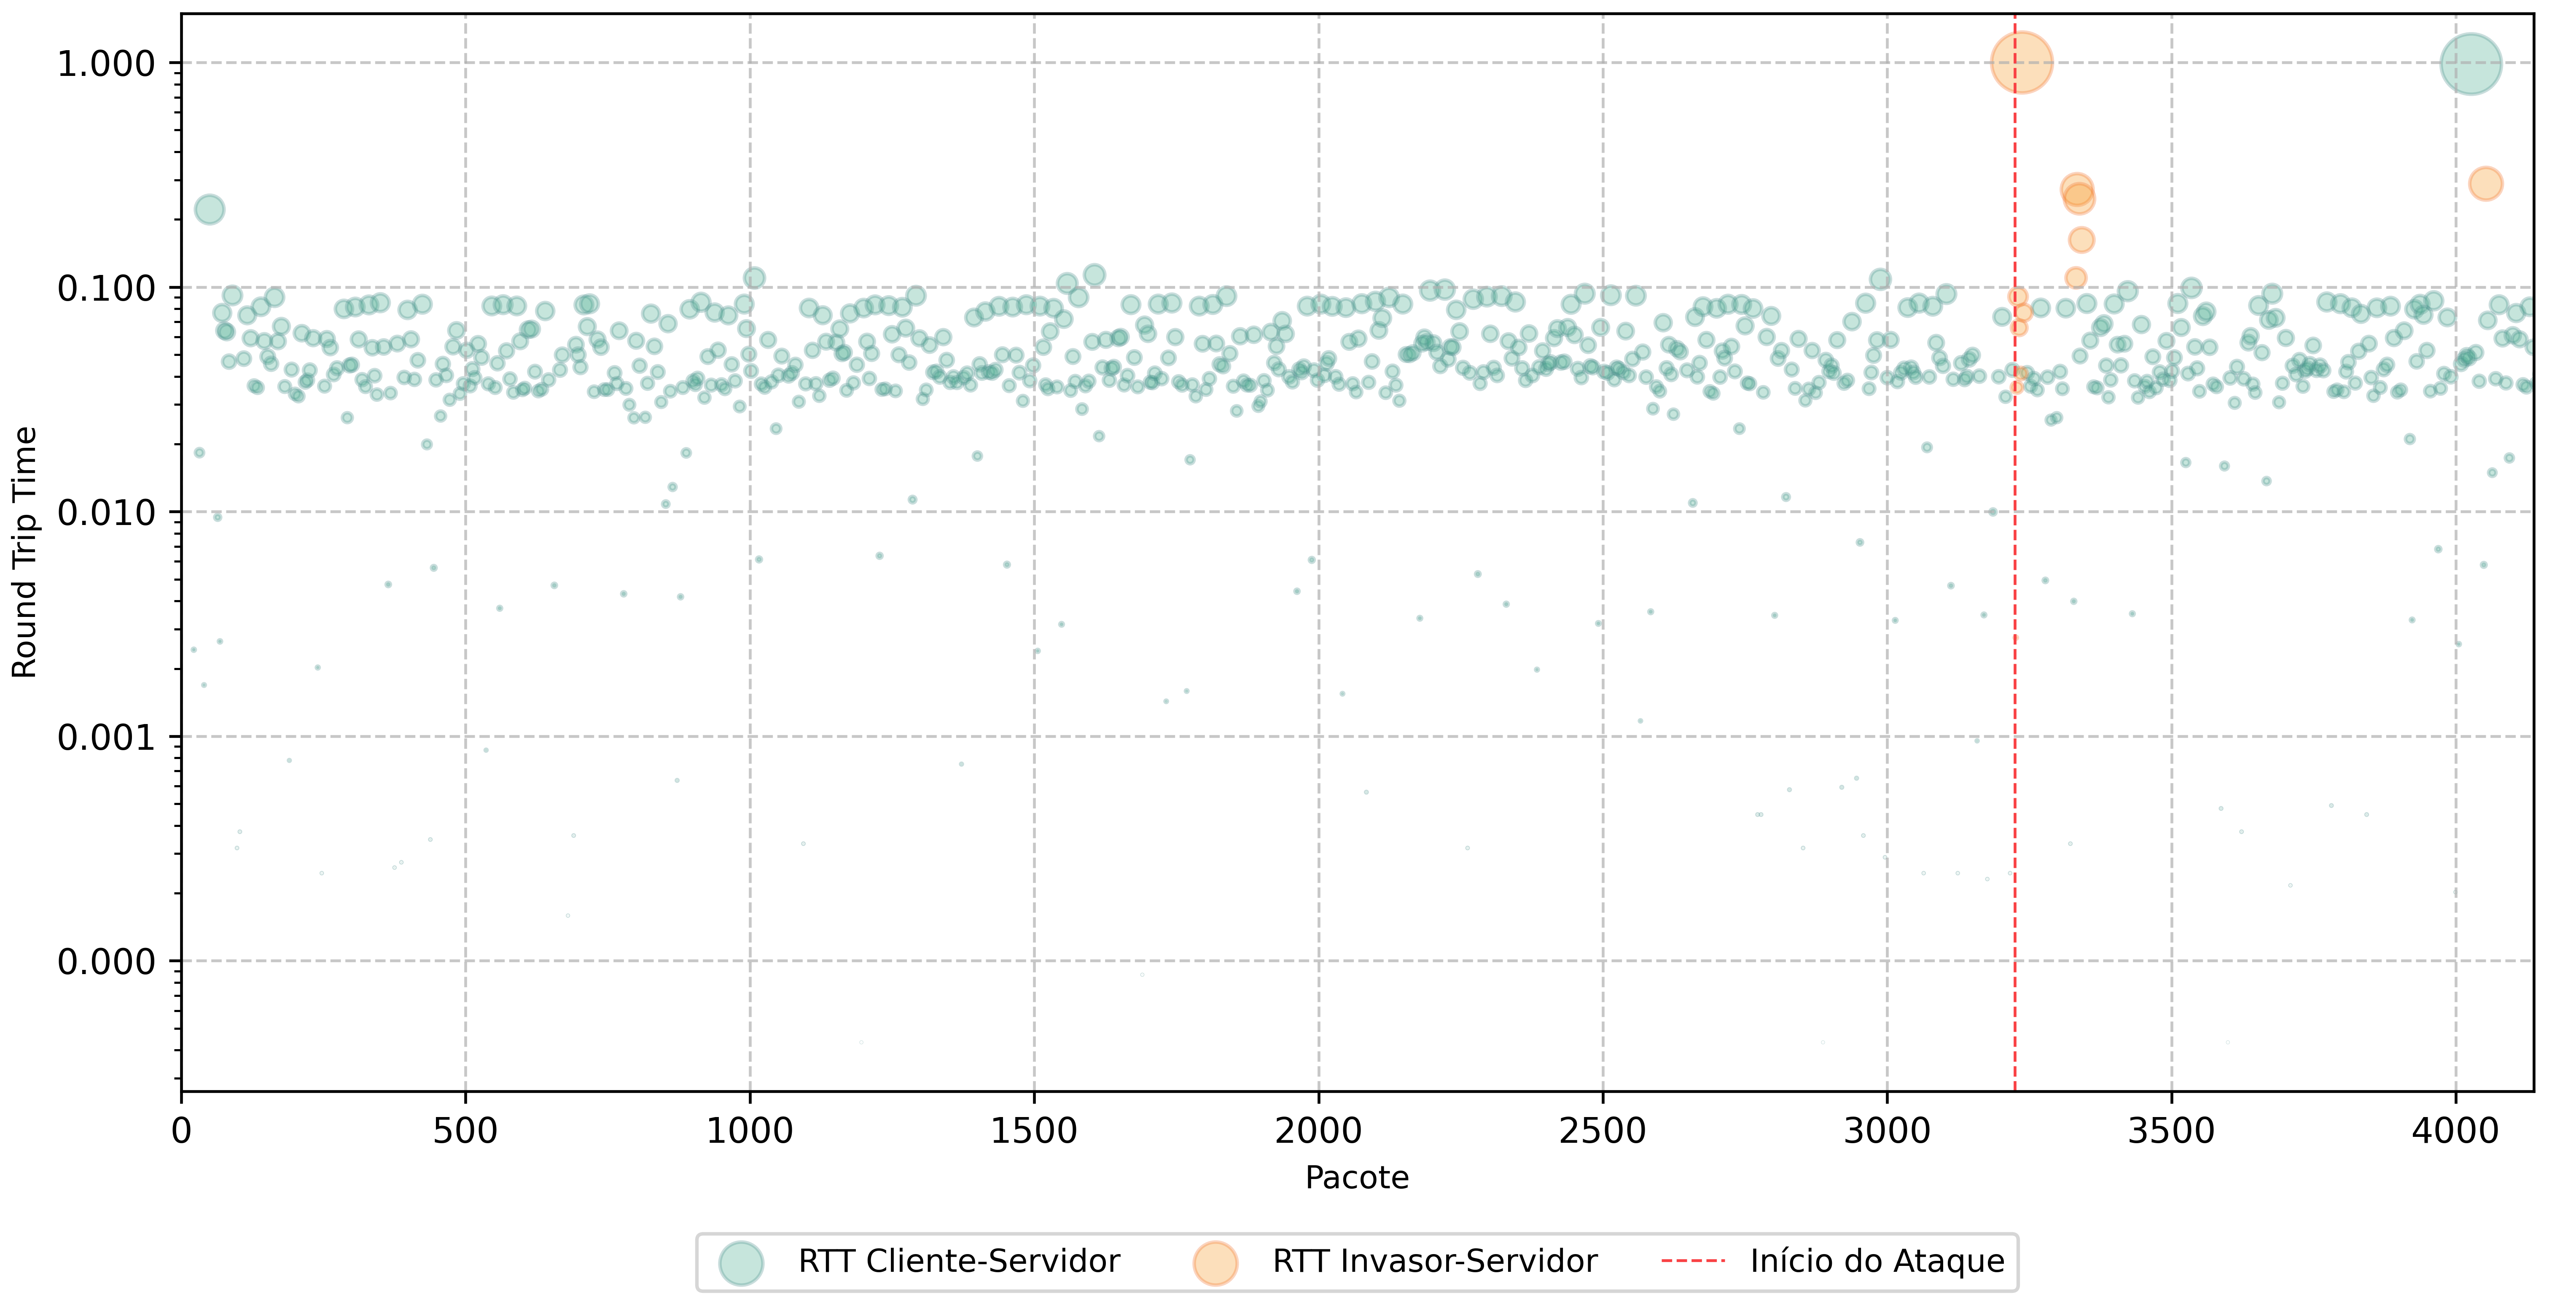
\includegraphics[width=0.972\textwidth]{USPSC-img/output/cropped/2-dos_certificate_inf_chain_loop-rttp.png}
    \end{center}
    \legend{Fonte: elaborada pelo autor.}
\end{figure}

A análise dos resultados revela uma interação do invasor com o servidor OPC UA apenas no momento do início do ataque. A comunicação a partir desse ponto é encerrada, para todos os modos de segurança, como indicado pela linha vermelha pontilhada que marca o início do ataque. Antes do ataque, o RTT Cliente-Servidor se mantém constante e estável. Entretanto, após o início do ataque, observa-se um aumento no RTT Invasor-Servidor, indicando que o servidor está sendo inundado com solicitações que levam ao aumento do tempo de resposta.

O gráfico também revela que, após o início do ataque, há uma dispersão significativa dos pontos de RTT Invasor-Servidor, o que sugere variações na capacidade do servidor de processar pacotes sob a carga do ataque. No entanto, o RTT Cliente-Servidor apresenta pouca variação, indicando que o servidor mantém a qualidade do serviço para comunicações legítimas, apesar da sobrecarga causada pelo ataque.

Essa análise reforça a eficácia do OPC UA em manter a resiliência contra ataques de negação de serviço, especialmente em cenários onde são implementadas medidas de segurança robustas, como o uso de criptografia e autenticação adequada. Além disso, destaca a importância de monitorar continuamente o desempenho do servidor e implementar mecanismos de mitigação de ataques para garantir a continuidade do serviço e a integridade dos dados. 

\subsubsection*{\underline{Chamada da função Dereference nula}}

O ataque de DoS pela chamada da função Dereference nula revelou-se o único capaz de causar uma negação de serviço completa na rede OPC UA industrial, para todos os diferentes cenários (C4, C5 e C6). Este ataque explora uma vulnerabilidade crítica no servidor, na qual uma chamada de função é executada sem verificar a validade do ponteiro, resultando em uma falha que pode travar o servidor. A técnica aproveita de vulnerabilidades na desreferenciação de um ponteiro nulo, que ocorre quando um programa tenta acessar ou modificar um ponteiro que, em vez de apontar para uma localização válida na memória, possui um valor nulo. A consequência imediata é que o programa tenta ler ou escrever em uma área de memória inválida, levando a uma interrupção abrupta do funcionamento do sistema. A gravidade desta falha reside no fato de que, além de interromper o serviço, ela pode ser explorada por atacantes para comprometer a segurança e a integridade do sistema, explorando comportamentos indefinidos que podem permitir a execução de código malicioso, ou levar a negação de serviço, como neste caso.

A análise dos gráficos fornecidos pela \autoref{fig:2-dos_null_deref} oferece uma compreensão detalhada do impacto deste ataque, especificamente para a rede configurada com modo de segurança `Sign \& Encrypt'.

\begin{figure}[htbp!]
    \centering
    \caption{\label{fig:2-dos_null_deref}Gráficos do ataque de DoS pela chamada da função \textit{Dereference} nula - nível de segurança: `Sign \& Encrypt'.}
    \begin{subfigure}[t]{0.5\textwidth}
        \centering
        \caption{\label{fig:2-dos_null_deref-tput}\textit{Throughput}}
        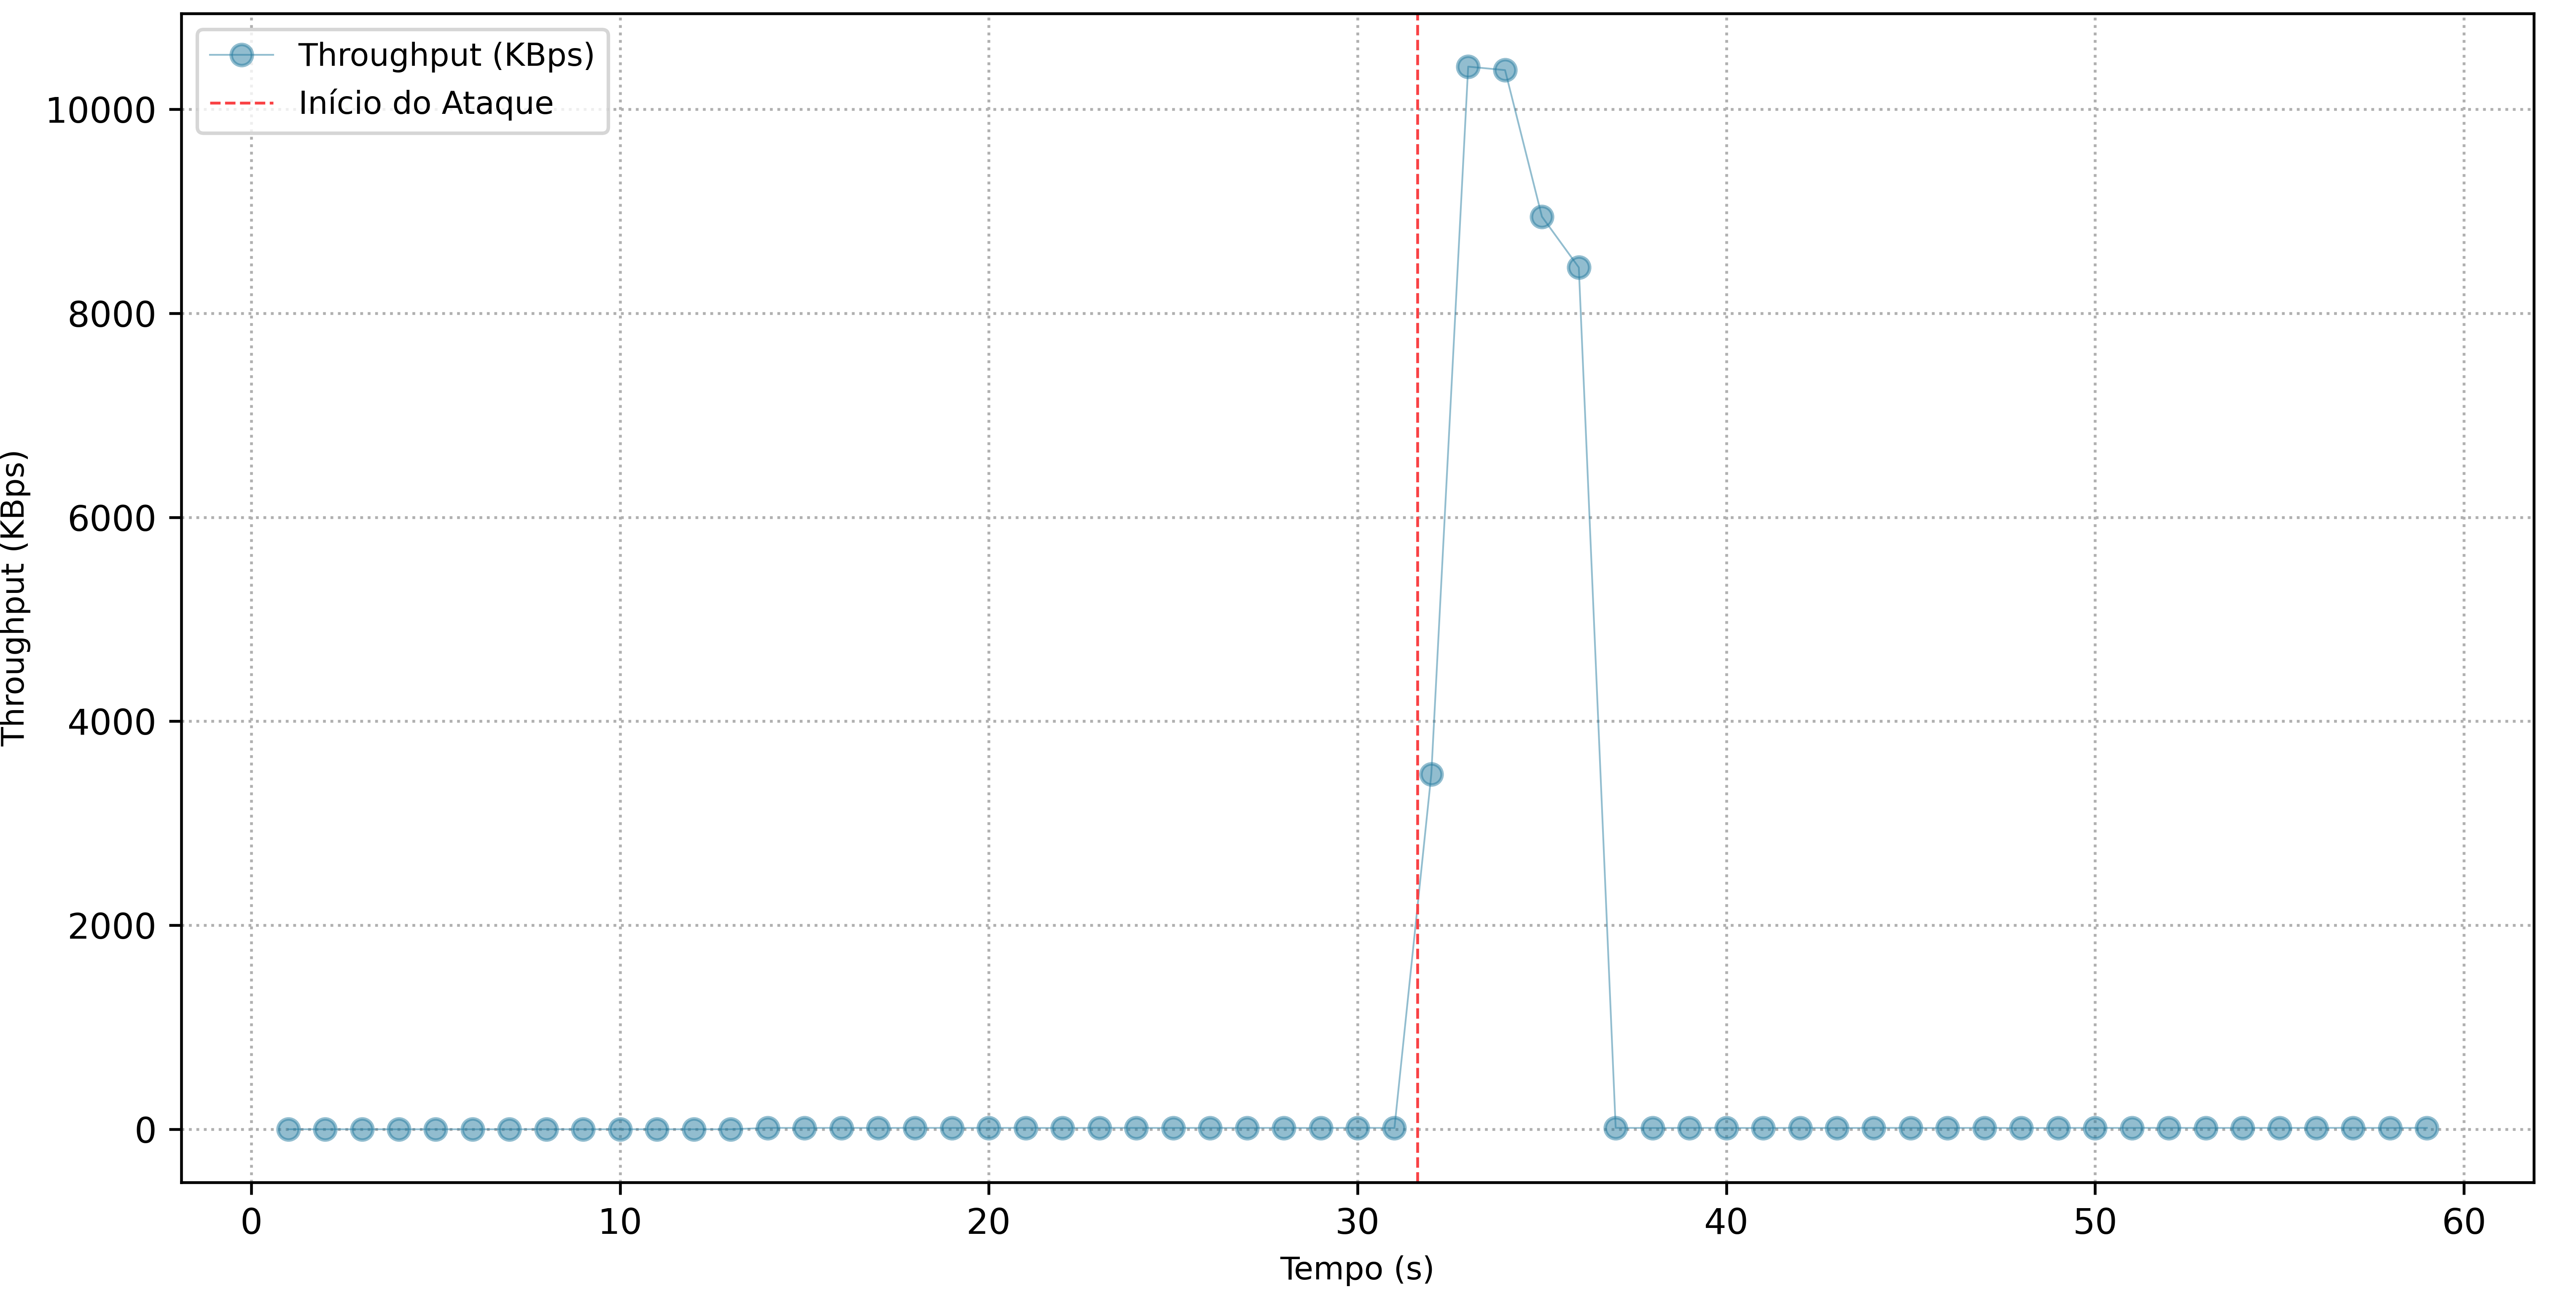
\includegraphics[width=1\textwidth, height=120pt]{USPSC-img/output/cropped/2-dos_function_call_null_deref-tput.png}
    \end{subfigure}%
    ~ 
    \begin{subfigure}[t]{0.5\textwidth}
        \centering
        \caption{\label{fig:2-dos_null_deref-perf}Desempenho}
        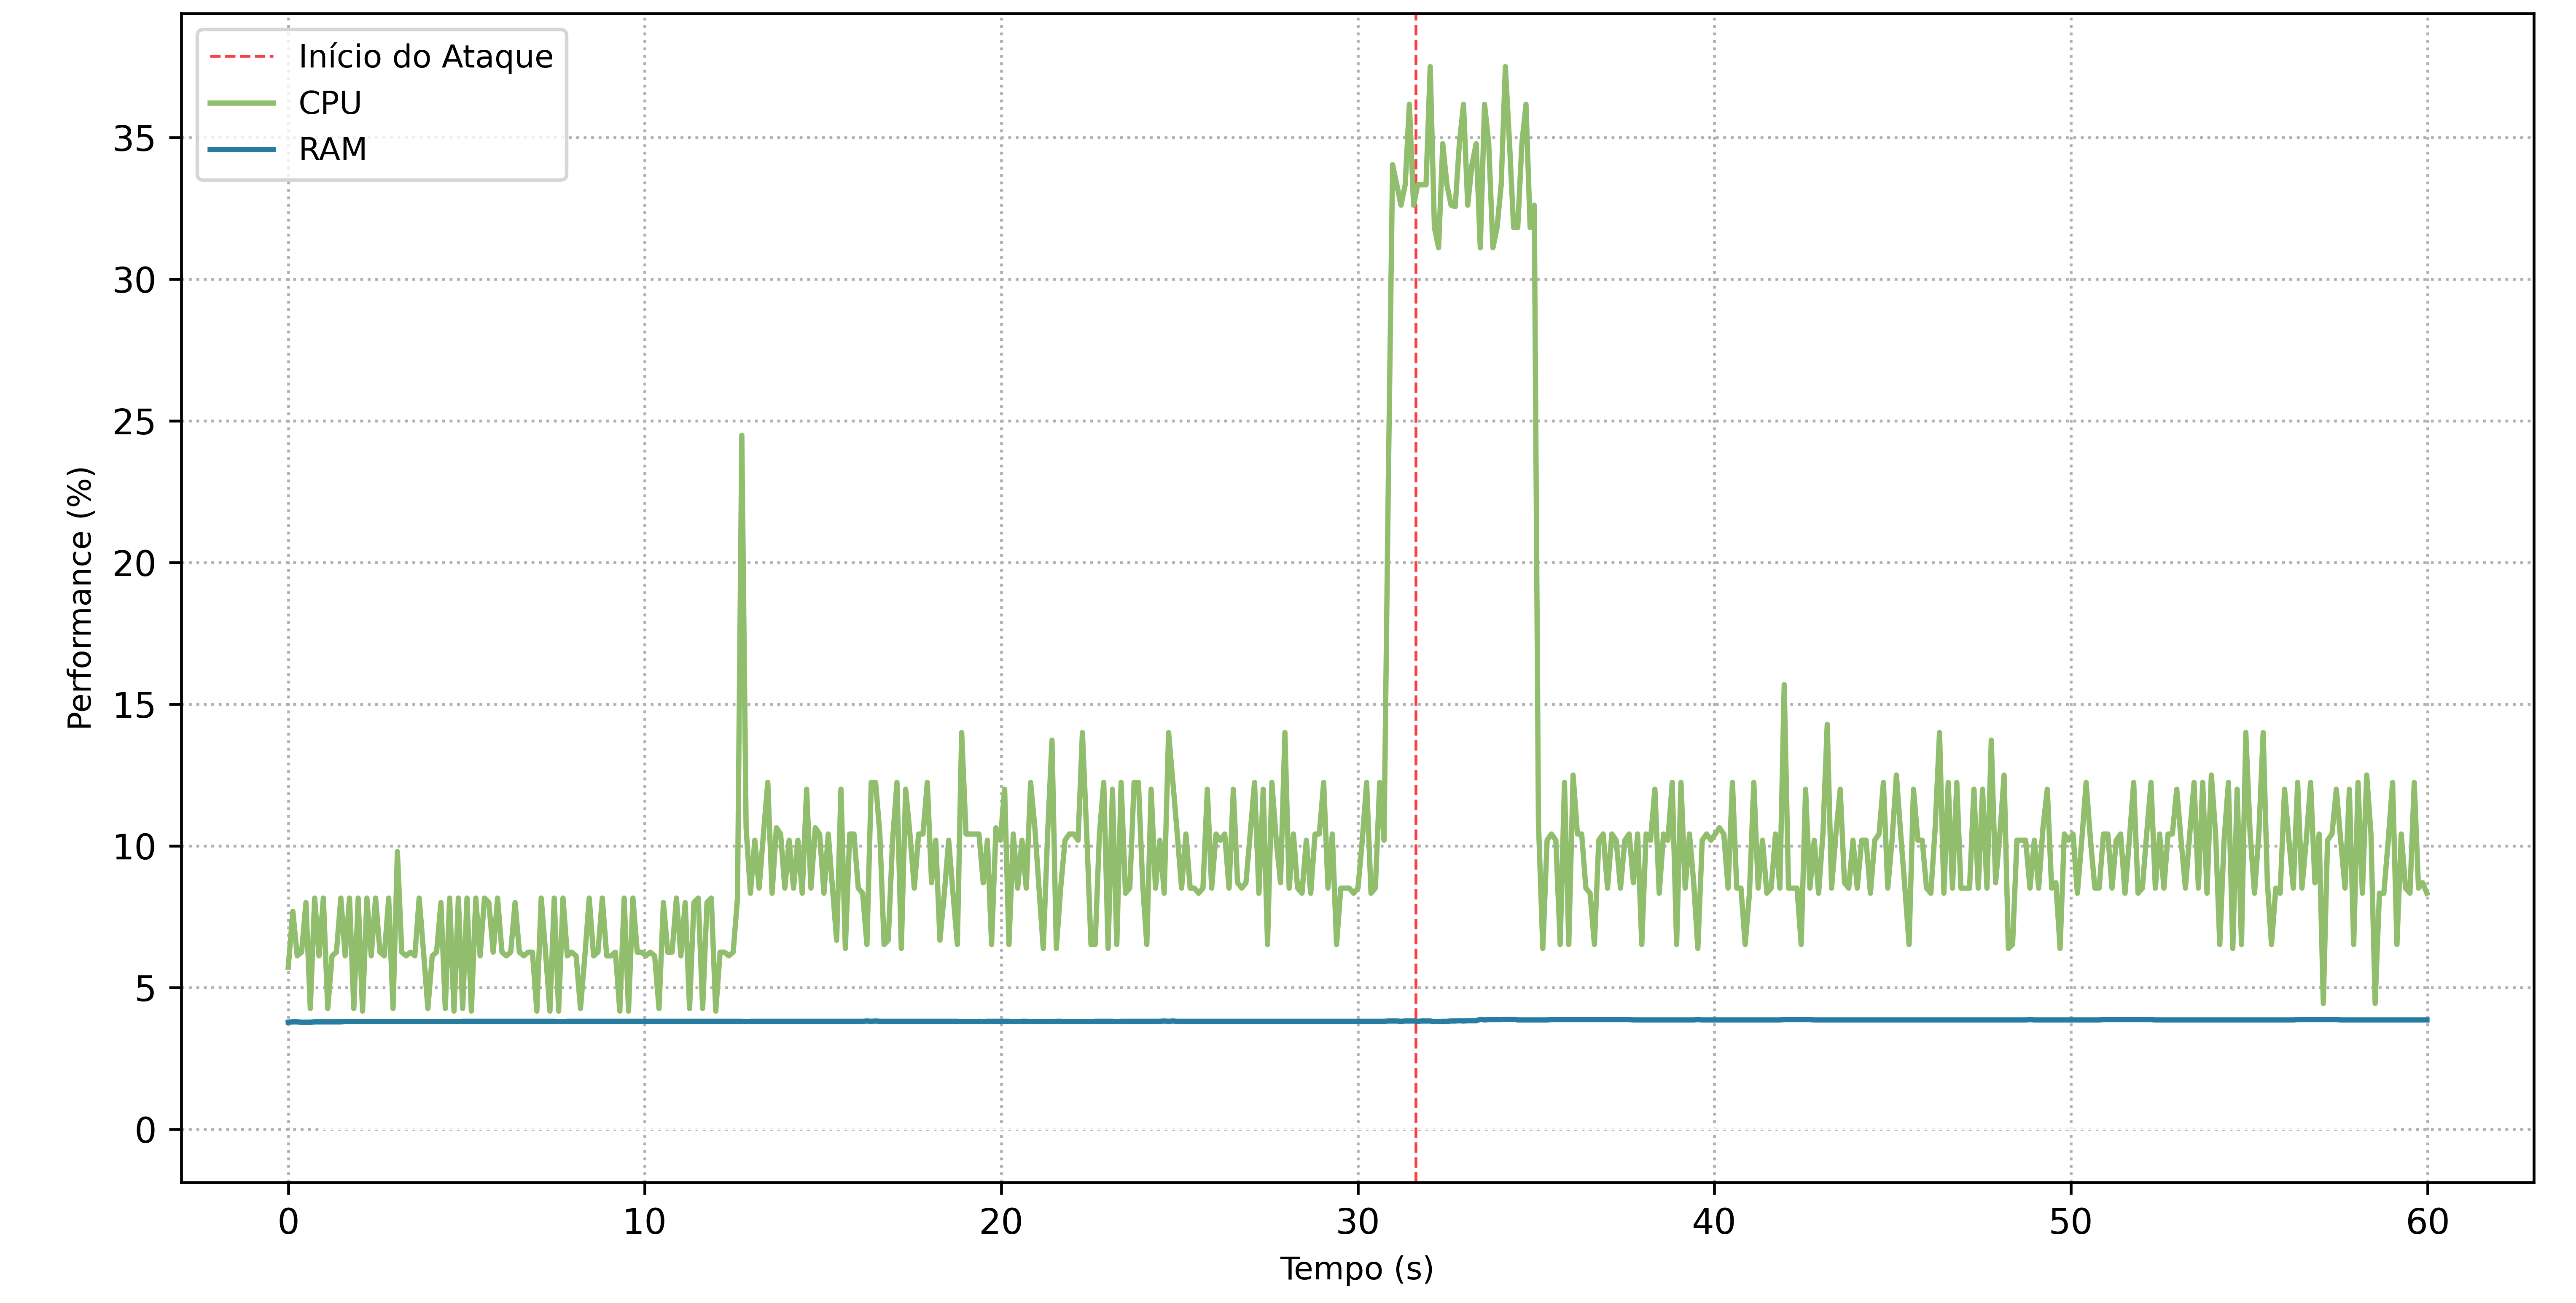
\includegraphics[width=1\textwidth, height=120pt]{USPSC-img/output/cropped/2-dos_function_call_null_deref-perf.png}
    \end{subfigure}%
    \\
    \begin{subfigure}[t]{0.5\textwidth}
        \centering
        \caption{\label{fig:2-dos_null_deref-pack}Pacotes OPC UA}
        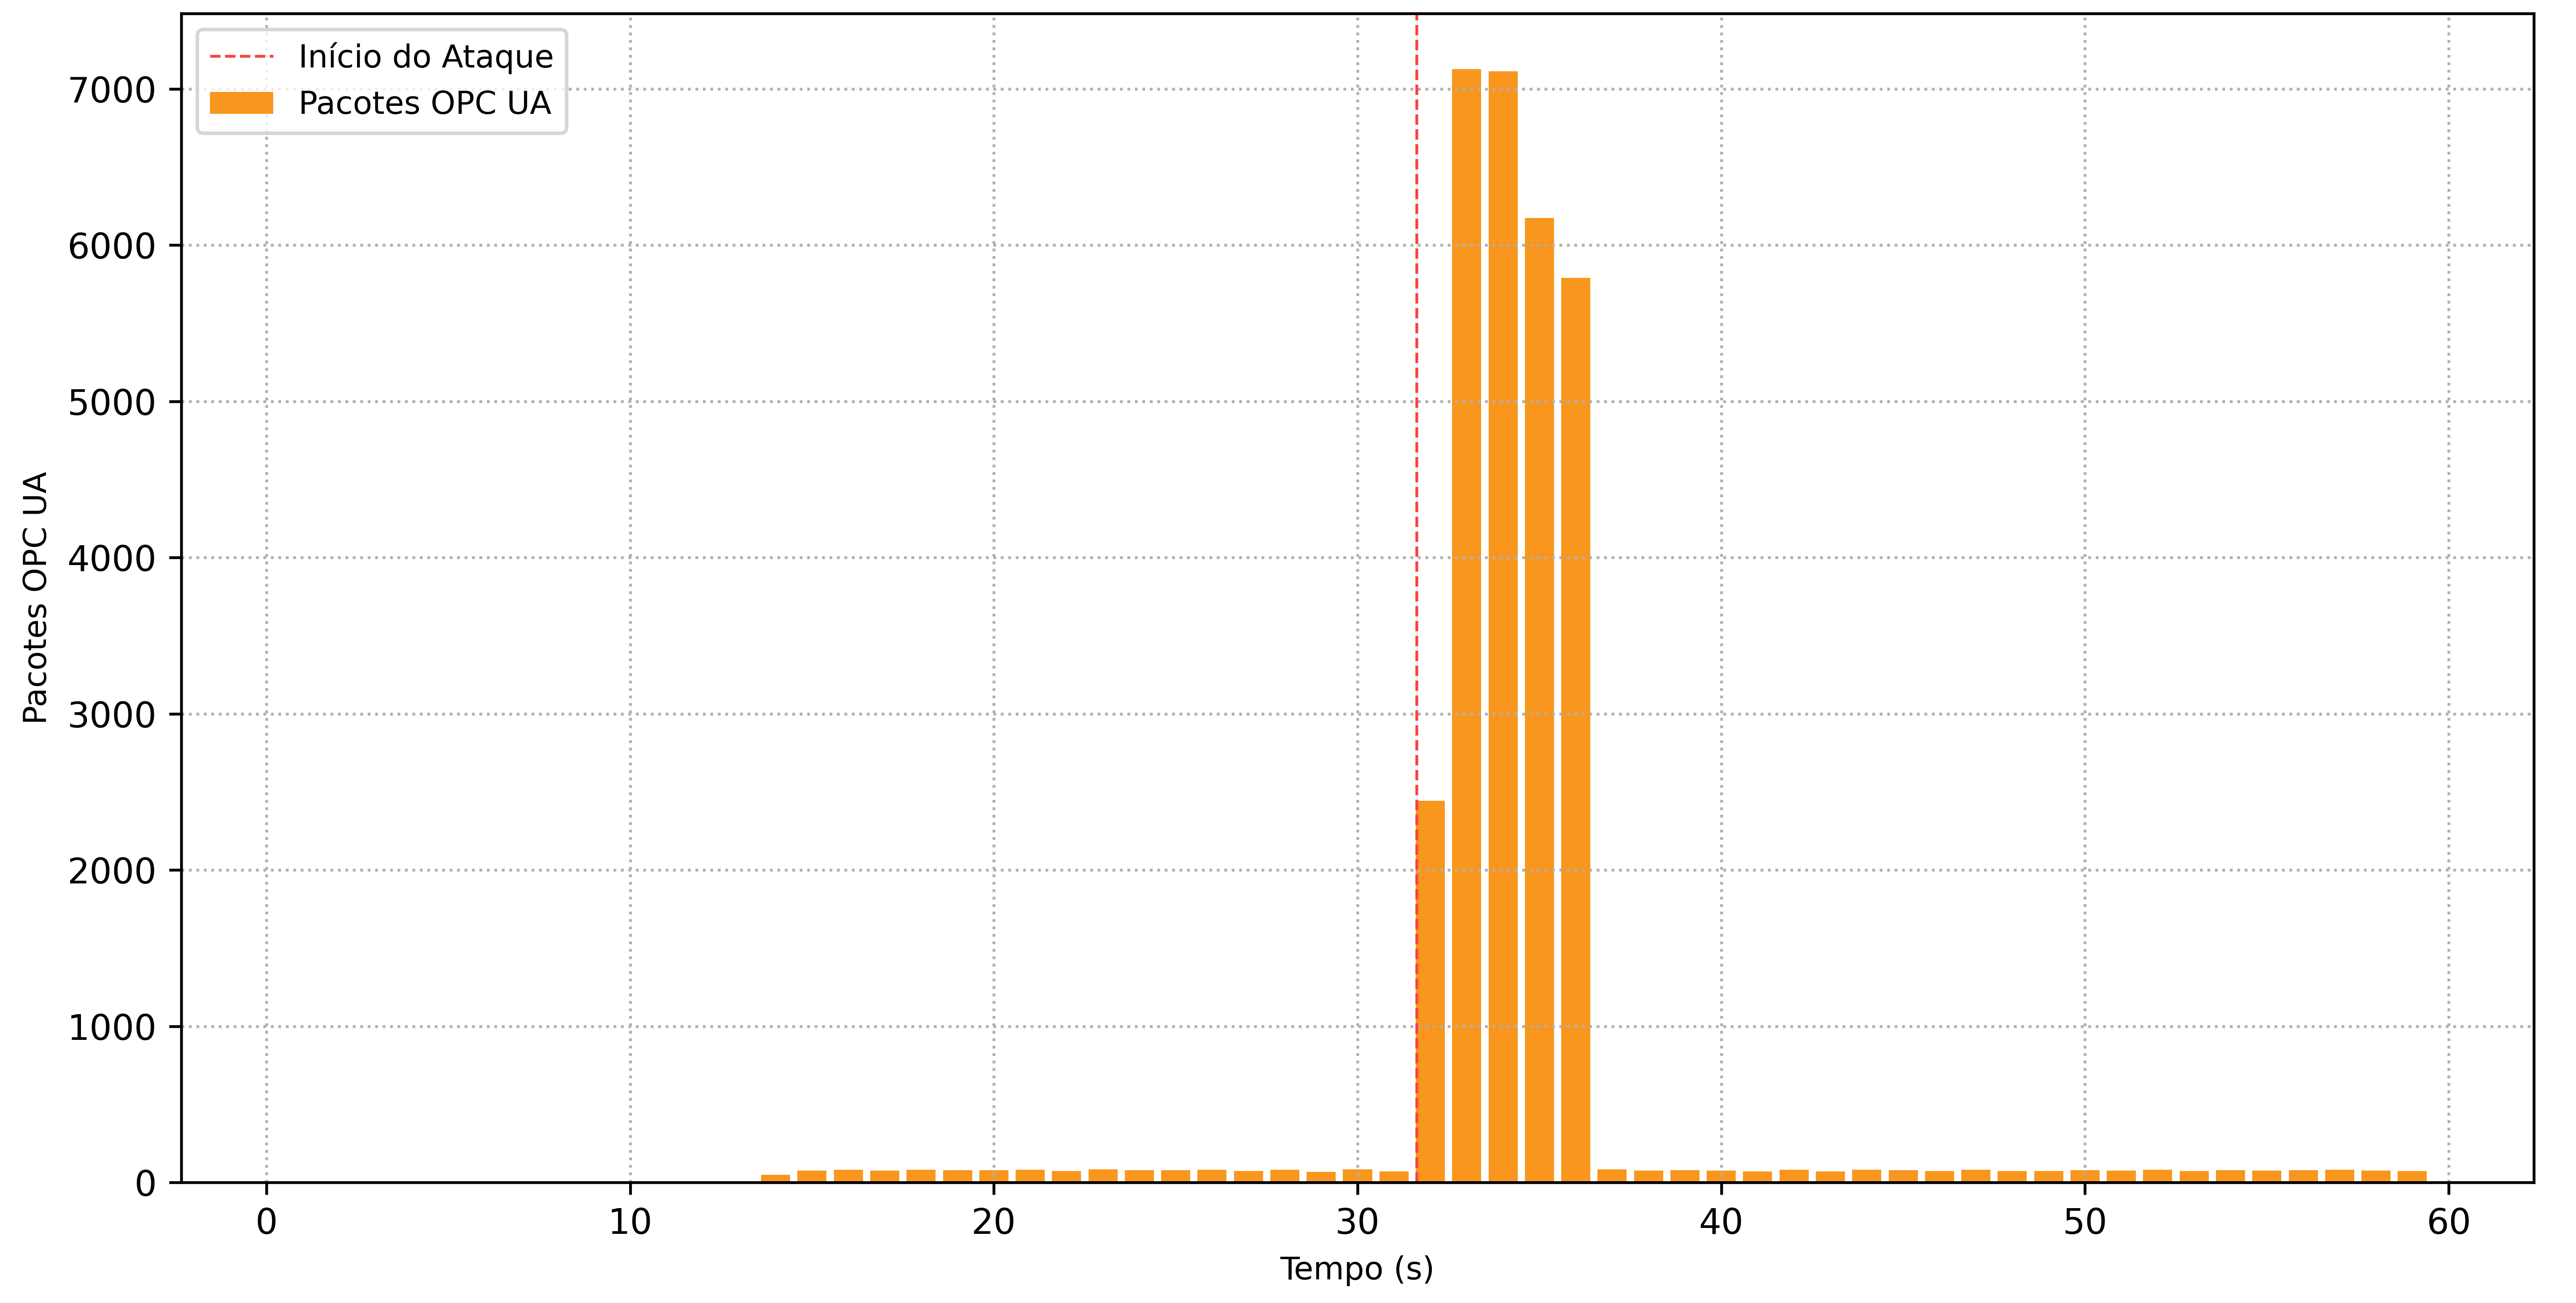
\includegraphics[width=1\textwidth, height=120pt]{USPSC-img/output/cropped/2-dos_function_call_null_deref-pack.png}
    \end{subfigure}%
    ~
    \begin{subfigure}[t]{0.5\textwidth}
        \centering
        \caption{\label{fig:2-dos_null_deref-rttp}RTT por pacote}
        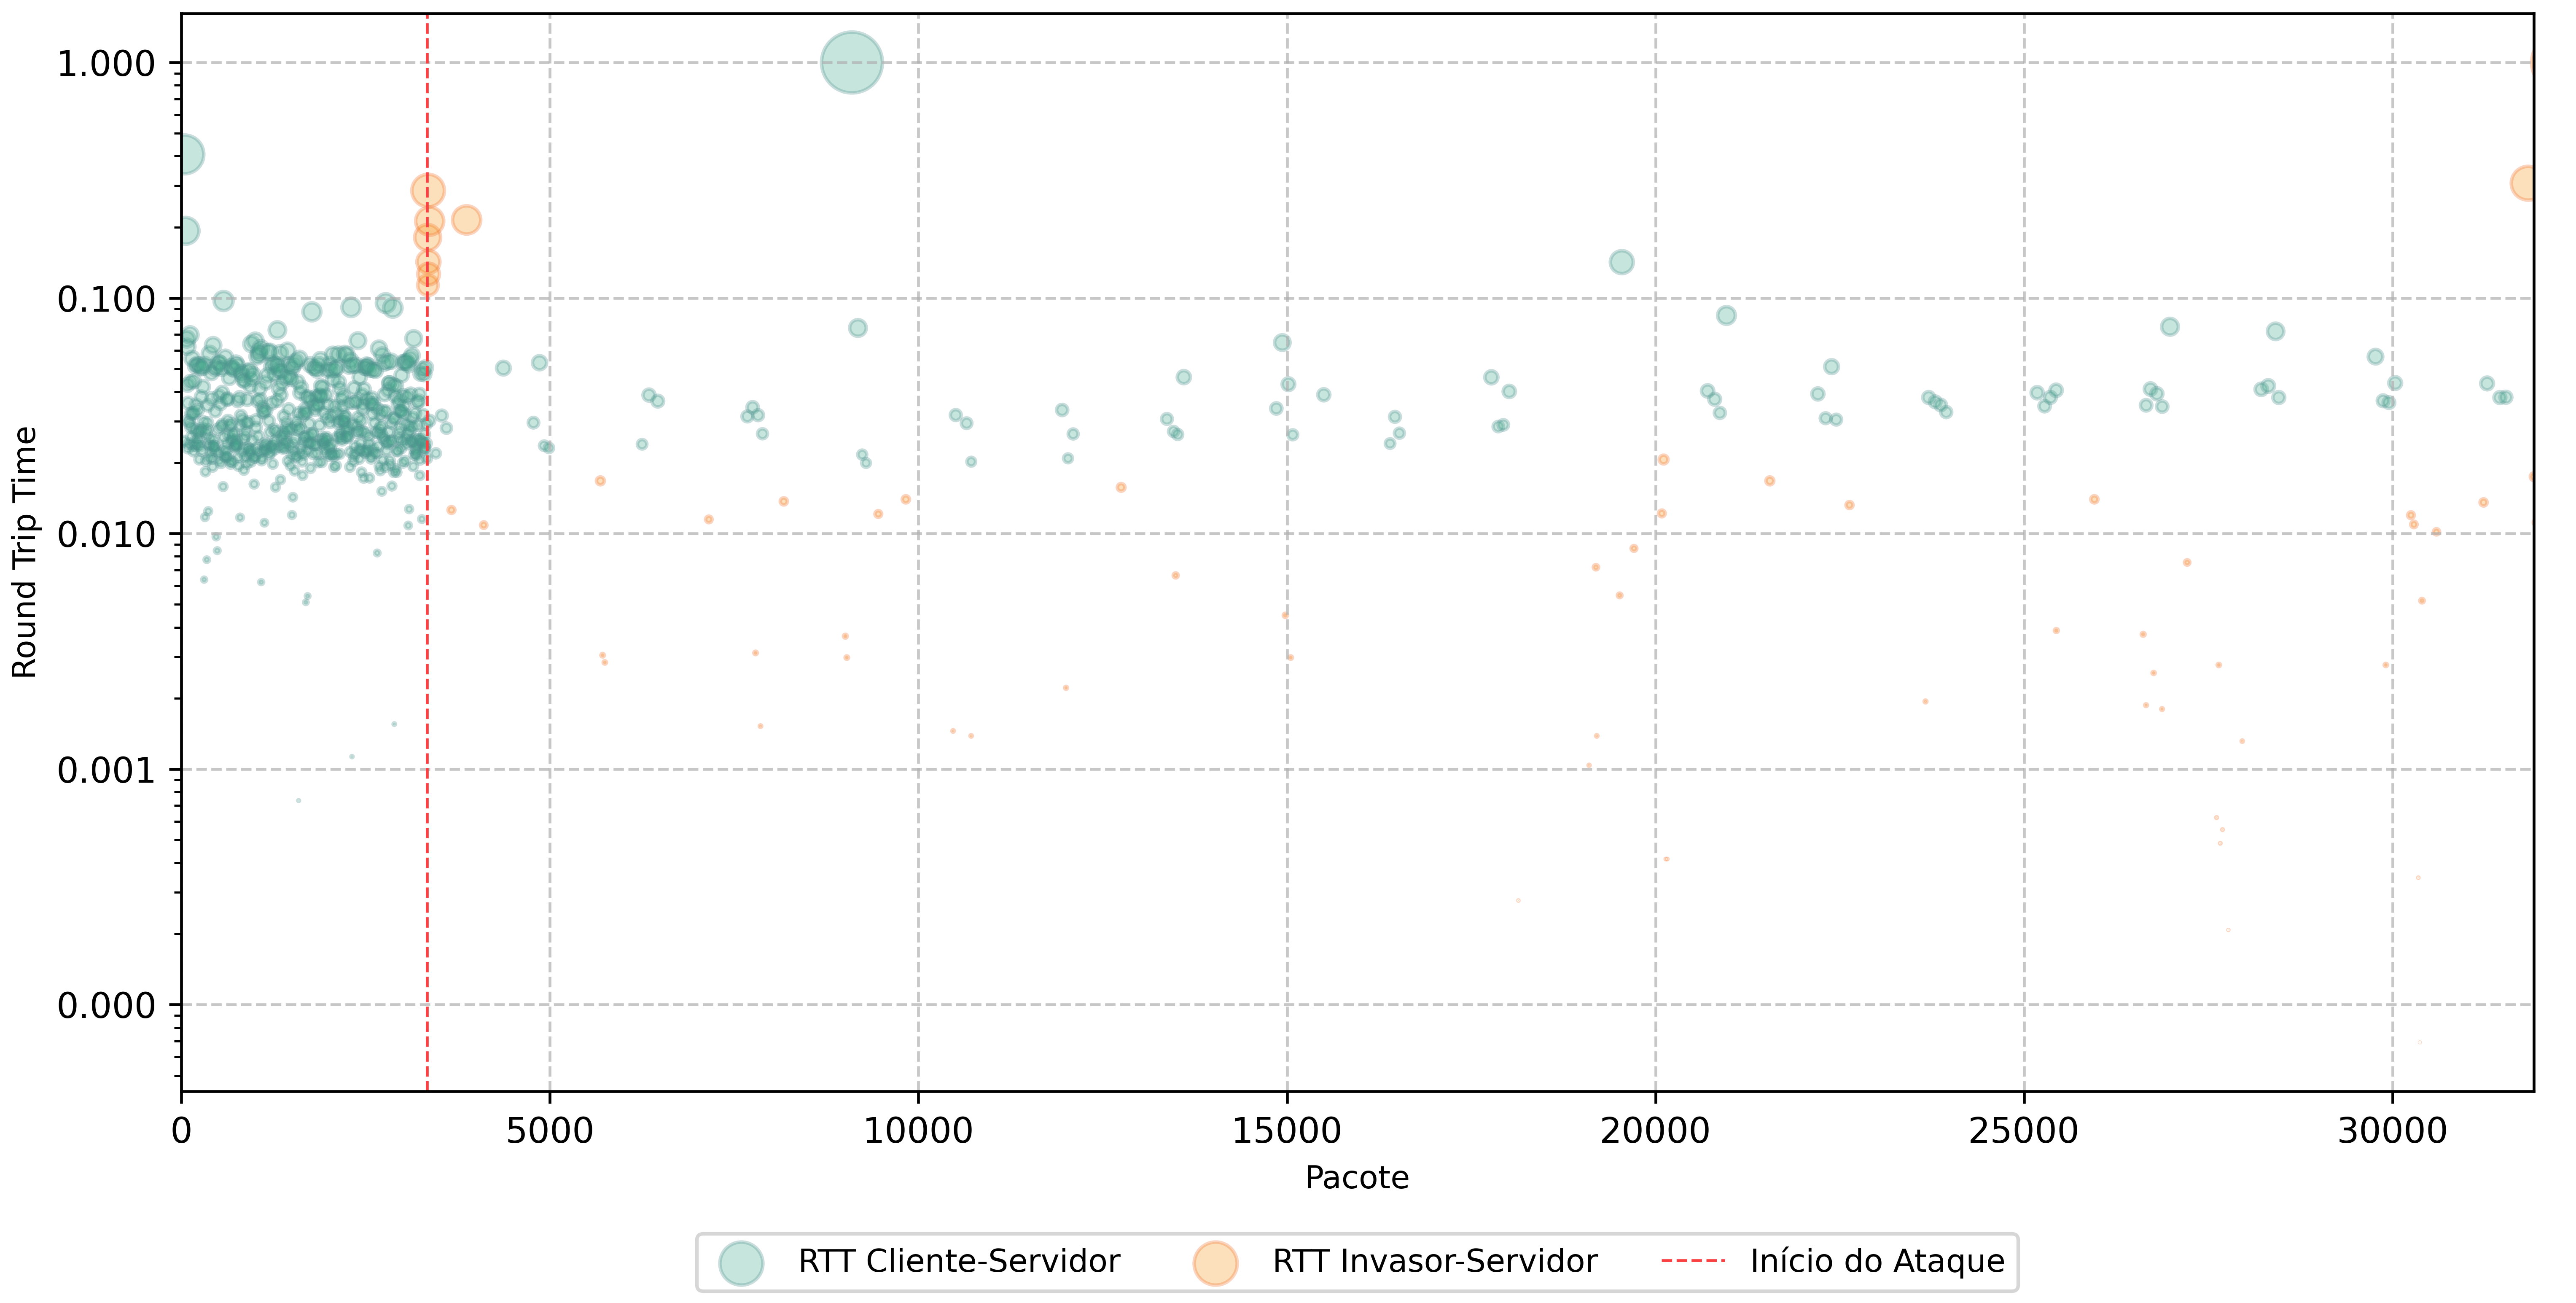
\includegraphics[width=1\textwidth, height=120pt]{USPSC-img/output/cropped/2-dos_function_call_null_deref-rttp.png}
    \end{subfigure}%
\end{figure}

O gráfico de taxa de transferência, representado na \autoref{fig:2-dos_null_deref-tput}, demonstra uma estabilidade em níveis baixos antes do ataque. Com o início do ataque, indicado pela linha vermelha, observa-se um aumento abrupto no throughput, atingindo um pico significativo antes de cair drasticamente a zero. Este comportamento indica que o servidor OPC UA foi sobrecarregado com solicitações inválidas, resultando em uma falha completa da comunicação, o que caracteriza uma negação de serviço.

A análise do gráfico de tempo de resposta por pacote, ilustrado na \autoref{fig:2-dos_null_deref-rttp}, corrobora esses achados. Antes do ataque, o RTT entre cliente e servidor permanece relativamente constante, refletindo uma comunicação estável. No entanto, com o início do ataque, há um aumento significativo no RTT, especialmente na comunicação entre o invasor e o servidor. Essa elevação súbita no RTT sugere que o servidor está demorando mais para processar as solicitações devido à sobrecarga provocada pelo ataque, culminando em um colapso na comunicação.

O impacto do ataque na performance do servidor é ainda mais evidente na \autoref{fig:2-dos_null_deref-perf}, que mostra o desempenho do host em termos de utilização de CPU e memória RAM. Antes do ataque, o uso da CPU se mantém em níveis baixos e constantes, indicando um funcionamento normal do servidor. No entanto, após o início do ataque, a utilização da CPU aumenta drasticamente, enquanto a utilização da RAM se mantém estável. Esta alta utilização da CPU é um indicativo claro de que o servidor está sobrecarregado tentando processar a grande quantidade de solicitações inválidas geradas pelo ataque, levando a uma queda de desempenho e, eventualmente, à falha do sistema.

Esses resultados demonstram que o ataque de chamada da função dereference nula é altamente eficaz em explorar vulnerabilidades específicas do servidor OPC UA, resultando em uma negação de serviço completa. A incapacidade do servidor de verificar a validade dos ponteiros antes de executar chamadas de função crítica foi o fator chave que permitiu a execução bem-sucedida deste ataque. A rápida elevação na utilização da CPU e a subsequente falha na comunicação destacam a necessidade urgente de medidas de mitigação para proteger servidores OPC UA contra tais vulnerabilidades.

\subsubsection*{\underline{Abertura de múltiplos canais seguros}}

A análise dos ataques DoS por meio da abertura de múltiplos canais seguros na comunicação OPC UA revela a gravidade dessa vulnerabilidade e seu impacto potencial em redes industriais. O ataque DoS (Denial of Service) explora a capacidade limitada de um servidor OPC UA para gerenciar múltiplos canais seguros, sobrecarregando-o e resultando em degradação ou interrupção do serviço. Esse tipo de ataque é particularmente preocupante em ambientes industriais, onde a comunicação contínua e segura é vital para o funcionamento de sistemas críticos.

Os resultados dos experimentos demonstram que a abertura simultânea de múltiplos canais seguros pode levar a um aumento significativo no throughput e no tempo de resposta, bem como na utilização da CPU. O gráfico de throughput mostra um aumento acentuado logo após o início do ataque, evidenciando que o servidor é incapaz de processar eficientemente a carga adicional de canais seguros. Esse aumento no throughput pode ser interpretado como uma tentativa do servidor de lidar com as múltiplas requisições, mas que acaba por sobrecarregar sua capacidade de processamento.

No gráfico de Round Trip Time (RTT), observa-se um aumento substancial no tempo de resposta após o início do ataque. Os pacotes entre o cliente e o servidor apresentam um aumento considerável no RTT, indicando que o servidor está sobrecarregado e não consegue responder prontamente às requisições. Além disso, a presença de pacotes do invasor com altos RTTs reforça a ideia de que o servidor está sendo incapaz de manter a eficiência sob ataque.

A análise do desempenho do host, especificamente da CPU e da RAM, também revela os efeitos adversos desse tipo de ataque. O gráfico de desempenho mostra um aumento considerável no uso da CPU após o início do ataque, enquanto o uso de RAM permanece estável. Isso sugere que a carga computacional imposta pela criação e manutenção de múltiplos canais seguros é a principal responsável pela degradação do desempenho do servidor.

Em conclusão, o ataque DoS por abertura de múltiplos canais seguros na comunicação OPC UA é uma vulnerabilidade séria que pode comprometer a integridade e a disponibilidade de sistemas industriais. A capacidade do servidor de lidar com uma carga elevada de canais seguros é limitada, resultando em um aumento no throughput, tempo de resposta e utilização da CPU, o que pode levar à interrupção do serviço. Portanto, é crucial que medidas de mitigação sejam implementadas para proteger redes OPC UA contra esse tipo de ataque.

\subsubsection*{\underline{Tradução do caminho de navegação}}

Uma vulnerabilidade crítica que pode ser explorada para comprometer a estabilidade e a segurança da rede OPC UA é a exaustão da pilha de função que processa requisições de tradução de caminhos de navegação para \texttt{NodeIds} (\texttt{TranslateBrowsePathsToNodeIds}). A função \texttt{TranslateBrowsePath} é responsável por traduzir caminhos de navegação (do inglês \textit{browse paths}) em \texttt{NodeIds}. Durante esse processo, a função é chamada recursivamente para cada elemento no caminho relativo (\texttt{RelativePath}), sem um limite adequado para a profundidade da recursão. Como resultado, a tradução de um caminho de navegação excessivamente longo pode levar a uma exceção de estouro de pilha (\texttt{StackOverflowException}).

No entanto, a análise dos resultados obtidos para estes cenários: C13, C14 e C15, revela que a rede OPC UA apresenta uma leve proteção contra ataques de negação de serviço por exaustão da pilha de função. A análise dos gráficos de dados do tráfego da rede, especificamente o tempo de resposta do servidor, revela uma degradação significativa no desempenho do sistema ao longo do tempo, no qual observa-se um aumento de forma acentuada à medida que o número de requisições maliciosas foi incrementado.


\section{Propostas de Melhorias e Mitigações} \label{sec:melhorias-mitigacoes}

A melhoria da resiliência cibernética de um IACS deve ser um dos muitos benefícios obtidos por meio da implementação de um programa de segurança industrial. Essa resiliência é alcançada quando os controles de segurança são selecionados de modo a abranger o processo contínuo de abordar a cibersegurança, que não apenas começa com a dissuasão e prevenção de ameaças, mas também equilibra de forma adequada a detecção e correção de ameaças. Isso é necessário para identificar eventos cibernéticos de maneira oportuna e responder adequadamente, a fim de minimizar as consequências do evento e devolver a instalação de manufatura à operação normal de forma segura e eficiente.

As organizações frequentemente dedicam grandes partes de seu orçamento de segurança a mecanismos de prevenção de ataques. No entanto, muitas vezes, são notificadas por partes externas sobre a falta de investimento equilibrado em controles para detectar um evento de violação, muito tempo após o ataque ter ocorrido. A segurança deve ser considerada um investimento ``estratégico'' de longo prazo, em vez de uma despesa ``tática'' de curto prazo ou única. Aqueles que investem e constroem instalações de manufatura compreendem o ciclo de vida de longo prazo do investimento de capital, por isso faz sentido que a segurança industrial utilizada para proteger essas mesmas instalações seja tratada de maneira semelhante, recebendo atenção contínua (e orçamento) como outras despesas operacionais (manutenção, melhorias, treinamento, etc.).

A segurança das comunicações em redes industriais é de suma importância, especialmente no contexto do uso do protocolo OPC UA. A partir de uma série de testes realizados em conformidade com os padrões de segurança, foram identificadas diversas recomendações que visam mitigar vulnerabilidades e fortalecer tanto a integridade quanto a confidencialidade dos dados.

Nesta seção, estão apresentadas as propostas de melhorias e mitigações identificadas, dividindo-as em duas categorias principais: as recomendações para comunicações seguras com o protocolo OPC UA e as melhorias na infraestrutura e destão de redes. Ao implementar essas recomendações, espera-se não apenas aumentar a robustez das comunicações, mas também assegurar a continuidade das operações industriais de forma segura e eficiente.

\subsection{Recomendações para Comunicações Seguras com o Protocolo OPC UA}

Em primeiro lugar, a operação no ``SecurityMode'' adequado é fundamental. Deve-se sempre optar pelos modos Sign' ou Sign \& Encrypt' para garantir que, no nível da aplicação, a autenticação seja obrigatória. O modo de segurança None' não oferece proteção e, portanto, não deve ser utilizado. O modo Sign \& Encrypt' é particularmente importante, pois assegura tanto a integridade quanto a confidencialidade dos dados transmitidos, prevenindo a interceptação e modificação não autorizada das informações.

A escolha dos algoritmos criptográficos também desempenha um papel crucial na segurança das comunicações OPC UA. Recomenda-se a utilização da Security Policy Basic256Sha256, desde que compatível com os clientes interagentes. Políticas de segurança que utilizam algoritmos desatualizados, como o SHA-1, devem ser evitadas, pois não proporcionam um nível de segurança adequado para as atuais ameaças cibernéticas.

No que diz respeito à autenticação de usuários, é essencial evitar o uso de logins anônimos para acessar recursos críticos. Utilizar um ID anônimo impossibilita o rastreamento de alterações nos dados ou configurações, abrindo brechas para atividades não autorizadas. Hackers podem explorar esta vulnerabilidade, comprometendo a segurança dos dados. Portanto, deve-se configurar restrições rigorosas para o uso de identificadores anônimos, garantindo que apenas operações não críticas sejam realizadas sob tais condições.

A proteção das chaves privadas e certificados é outro aspecto vital. Esses elementos não devem ser armazenados em sistemas de arquivos não criptografados. Devem-se utilizar os armazenamentos de certificados dos sistemas operacionais, que permitem definir direitos de acesso apropriados. Além disso, o uso de TPMs (Trusted Platform Modules) ou de hardware seguro externo, como tokens de autenticação USB, é altamente recomendado para o armazenamento seguro de certificados e chaves privadas, reduzindo o risco de comprometimento desses ativos.

O uso de certificados confiáveis é imperativo. Conexões que não fornecem certificados confiáveis devem ser bloqueadas. Embora certificados autoassinados possam ser utilizados, eles requerem verificações adicionais. Preferencialmente, deve-se estabelecer uma autoridade certificadora (CA), cujos certificados devem ser assinados de forma independente ou por outra CA. Este modelo de confiança pode ser multinível, fortalecendo ainda mais a autenticidade das comunicações.

Finalmente, a gestão e manutenção de certificados são essenciais para manter a segurança contínua. A utilização de listas de confiança de certificados e listas de revogação de certificados permite gerenciar apenas certificados válidos. Essas listas, criadas por usuários ou processos confiáveis, devem ser atualizadas regularmente para assegurar que somente certificados legítimos sejam aceitos, prevenindo possíveis ataques de falsificação de identidade.

Essas medidas, quando implementadas de forma integrada, fornecem uma base robusta para a segurança das comunicações em redes industriais utilizando o protocolo OPC UA, mitigando riscos e assegurando a continuidade das operações críticas com integridade e confidencialidade.

\subsection{Melhorias na Infraestrutura e Gestão de Redes}

% MITM:

% Port stealing Port stealing - countermeasures - countermeasures
% n YES - port security on the switch - port security on the switch
% n NO - static ARP - static ARP

% ARP poison - countermeasures - countermeasures
% n YES - passive monitoring (arpwatch) - passive monitoring (arpwatch)
% n YES - active monitoring (ettercap) - active monitoring (ettercap)
% n YES - IDS (detect but not avoid) - IDS (detect but not avoid)
% n YES - Static ARP entries entries (avoid it) (avoid it)
% n YES - Secure-ARP (public - Secure-ARP (public key auth)
% n NO - Port security security on the on the switch
% n NO - anticap anticap, antidote, , antidote, middleware middleware approach approach

A segurança das redes de comunicação industrial é crucial para garantir a integridade, confidencialidade e disponibilidade dos dados. Ataques como Man-in-the-Middle (MITM), Sniffing e Denial of Service (DoS) representam ameaças significativas que podem comprometer a operação de sistemas críticos. A implementação de contramedidas eficazes e melhorias na infraestrutura e gestão de redes são essenciais para mitigar esses riscos e proteger os ativos de comunicação.

Os ataques MITM, incluindo port stealing e ARP poisoning, podem ser mitigados por meio de várias abordagens. A segurança de porta nos switches é uma medida fundamental para impedir que dispositivos não autorizados roubem portas para interceptar o tráfego de rede. Esta técnica limita o número de endereços MAC que podem ser aprendidos em cada porta e pode desativar portas automaticamente ao detectar violações, aumentando a segurança da rede. Além disso, a utilização de entradas ARP estáticas impede que dispositivos maliciosos alterem as tabelas ARP para redirecionar o tráfego, sendo uma abordagem eficaz em redes onde a topologia e os endereços IP são conhecidos e estáveis.

Para combater o ARP poisoning, várias técnicas de monitoramento são recomendadas. O monitoramento passivo com ferramentas como arpwatch permite a detecção de alterações suspeitas nas tabelas ARP, alertando os administradores sobre possíveis ataques. Ferramentas de monitoramento ativo, como o ettercap, são usadas para identificar e neutralizar atividades de ARP poisoning em tempo real. Além disso, a implementação de sistemas de detecção de intrusão (IDS) é crucial, pois esses sistemas monitoram o tráfego de rede em busca de padrões anômalos que indicam a presença de ataques MITM. No entanto, embora os IDS detectem ataques, eles não os impedem diretamente.

A adoção de Secure-ARP, que utiliza autenticação por chave pública, oferece uma solução robusta contra ARP poisoning, garantindo a integridade das entradas ARP. Essa abordagem é complementada pela definição de entradas ARP estáticas, embora esta possa ser uma tarefa administrativamente onerosa.

O sniffing, que envolve a captura não autorizada de tráfego de rede, pode ser mitigado através de várias técnicas. A criptografia de dados em trânsito utilizando protocolos seguros como TLS/SSL é fundamental para impedir que atacantes obtenham informações sensíveis, mesmo que consigam capturar o tráfego. A segmentação de rede, implementando VLANs, limita a exposição de dados a apenas os segmentos necessários, dificultando o acesso não autorizado ao tráfego de rede. A segurança de porta nos switches também desempenha um papel crucial aqui, impedindo que dispositivos não autorizados se conectem à rede e capturem tráfego.

Para mitigar ataques DoS, que visam interromper a disponibilidade dos serviços, diversas contramedidas são recomendadas. A implementação de filtros de tráfego nos roteadores e switches pode bloquear pacotes maliciosos antes que atinjam os servidores e dispositivos críticos. Sistemas de prevenção de intrusão (IPS) são igualmente importantes, pois, além de detectar, podem bloquear automaticamente o tráfego malicioso, impedindo que os ataques DoS atinjam seus objetivos. A capacidade de escalabilidade da infraestrutura de rede, com redundância e capacidade de absorção de picos de tráfego malicioso, é crucial para garantir a continuidade dos serviços.

O monitoramento contínuo da rede é essencial para identificar e responder rapidamente a padrões de tráfego anômalos, ajudando a mitigar os efeitos de um ataque DoS. A adoção de uma abordagem abrangente, que inclui medidas técnicas e boas práticas de gestão, é essencial para enfrentar as ameaças cibernéticas de forma eficaz e assegurar a resiliência das infraestruturas industriais.

% Eric D. Knapp - Industrial Network Security_ Securing Critical Infrastructure Networks for Smart Grid, SCADA, and Other Industrial Control Systems-Syngress (2024)

% De acordo com o Princípio da Menor Rota (veja o Capítulo 5, “Design e Arquitetura de Redes Industriais”), um dispositivo que não pertence fisicamente a uma zona não deve ser autorizado a conectar-se diretamente a essa zona ou a qualquer dispositivo dentro dela. Esta é a razão principal pela qual as redes consistem em uma ou mais “DMZs” semiconfiáveis, que atuam como uma conexão intermediária entre dispositivos que possuem objetivos funcionais tanto semelhantes quanto diferentes, enquanto residem em duas zonas distintas (por exemplo, um usuário empresarial que necessita de dados históricos do ICS).

% Em muitos casos, haverá dispositivos secundários identificados que têm acesso ou estão conectados a uma zona, como uma impressora ou dispositivo de armazenamento que pode fornecer conectividade de rede. Um exemplo é uma impressora de rede com interface Wi-Fi, que pode estar ativada por padrão. Essas aberrações são fáceis de ignorar, mas devem ser abordadas para que a zona seja segura. Esta é uma das razões pelas quais avaliações minuciosas de risco e vulnerabilidade de segurança precisam ser realizadas (veja o Capítulo 8, “Avaliações de Risco e Vulnerabilidade”).

% Pode não ser possível, em outros casos, identificar claramente os limites de uma zona em termos de design de rede. Por exemplo, se sistemas de supervisão, controle e empresariais estiverem todos interconectados por uma rede plana (uma rede comutada puramente na Camada 2, sem roteamento de rede) ou uma rede sem fio, não será possível isolar zonas através de sub-redes. Nesses casos, algum outro meio de segmentação lógica de rede deve ser utilizado. Por exemplo, VLANs podem ser usadas para separar dispositivos que estão em diferentes zonas, segmentando a rede na Camada 2 do modelo OSI. Outra abordagem poderia ser implementar uma tecnologia conhecida como ``máscara de sub-rede de comprimento variável'' (VLSM), que manipula os parâmetros de Máscara de Sub-rede e Gateway Padrão de uma interface de rede, restringindo os dispositivos que podem realmente se comunicar na camada de rede (Camada 3 do OSI) sem introduzir novos dispositivos na Camada 3. Alternativamente, um firewall de última geração poderia ser utilizado no conduto entre zonas para segmentar os dispositivos na Camada 7 do modelo OSI. Cada abordagem tem seus pontos fortes e, idealmente, a separação de zonas deveria ser aplicada em todas as sete camadas; se não houvesse restrições de orçamento e sobrecarga operacional, isso seria possível. Vale notar que o uso de VLANs e VLSM fornece apenas níveis moderados de defesa cibernética, conforme descrito no Capítulo 5, “Design e Arquitetura de Redes Industriais”, e não é recomendado para redes que exigem níveis mais altos de segurança, tipicamente alcançados por meio de mecanismos de segmentação física.

% O método a seguir é eficaz para a separação de zonas:

% \begin{itemize}
%     \item Identificação e documentação: Identificar e documentar todas as conexões de rede que entram ou saem de cada zona (ou seja, identificar pontos de entrada/saída que formam condutos).
%     \item Avaliação por camadas: Para cada conduto, começar na Camada 1 (física) e trabalhar até a Camada 7 (aplicação). Para cada camada, avaliar se a segmentação de rede nessa camada é viável para aquele conduto (veja o Capítulo 5, “Design e Arquitetura de Redes Industriais” para detalhes sobre segmentação de redes em diferentes camadas).
%     \item Segmentação crítica: Para condutos mais críticos, buscar uma segmentação maior—implementar segmentação de rede por meio do uso de uma mistura de diodo de dados ou gateway unidirecional na Camada 1, comutação e segmentação de aplicação nas Camadas 3-4, e firewalls de última geração nas Camadas 5-7.
%     \item Implementação de controles de segurança: Para cada camada desejada de segmentação, implementar controles de segurança de rede e de acesso apropriados para reforçar essa segmentação.
%     \item Monitoramento: Prover capacidades de monitoramento suficientes com cada controle de segurança implantado para suportar mecanismos de consolidação de eventos e relatórios que auxiliem em potenciais violações de segurança.
% \end{itemize}

% Estabelecer a segurança de rede para proteger o acesso a uma zona definida envolve, essencialmente, a imposição de condutos. As regras aplicadas estão alinhadas com os canais de comunicação contidos dentro desses condutos. Os controles de segurança de rede protegem contra acesso não autorizado aos sistemas internos e também impedem que esses sistemas acessem sistemas externos de dentro para fora. Para garantir a segurança efetiva do tráfego de entrada e saída, duas ações são necessárias:

% \begin{enumerate}
%     \item Todo o tráfego de entrada e saída deve ser direcionado através de uma ou mais conexões de rede conhecidas que sejam monitoradas e controladas.
%     \item Um ou mais dispositivos de segurança devem ser colocados em linha em cada uma dessas conexões (isso pode ser uma capacidade de segurança incorporada em switches e roteadores de comunicação de rede).
%     \item Para cada zona, os dispositivos de segurança apropriados devem ser selecionados e implementados de acordo com as recomendações a seguir.
% \end{enumerate}

% Seleção de Dispositivos de Segurança de Rede
% No mínimo, algum tipo de firewall de rede é geralmente necessário. Segurança adicional, fornecida por IDS, IPS e uma variedade de dispositivos especializados e híbridos, como dispositivos de Gerenciamento Unificado de Ameaças (UTM), dispositivos de Lista Branca de Rede, Monitores de Aplicações e Filtros de Protocolos Industriais, pode ser desejável dependendo da situação específica. Tipicamente, o nível de segurança ou criticidade da zona (ver “Criticidade”) dita o grau de segurança necessário. A Tabela 11.1 mapeia a criticidade de uma zona para as medidas de segurança exigidas pelo NERC CIP e NRC CFR 73.54, bem como melhorias recomendadas para melhorar a segurança além dos requisitos regulamentares.

% A Tabela 11.1 recomenda o uso de um firewall e um IPS em cada perímetro de segurança. Isso porque firewalls e dispositivos IPS têm funções diferentes. Firewalls impõem quais tipos de tráfego são permitidos passar pelo perímetro através do que é chamado de ``inspeção superficial de pacotes". Sistemas de prevenção de intrusão, por outro lado, realizam ``inspeção profunda de pacotes'' (DPI) examinando de perto o tráfego permitido para detectar tráfego ``legítimo'' com intenções maliciosas—como código de exploração, malware, etc.—que é transferido por caminhos permitidos. O uso conjunto de ambos os dispositivos proporciona dois benefícios mútuos: primeiro, permite que o IPS inspecione o ``conteúdo'' de todo o tráfego permitido pelo firewall; segundo, o firewall limita o tráfego permitido com base nos parâmetros definidos da zona de segurança, liberando o IPS para focar seus recursos apenas nesse tráfego, permitindo assim a aplicação de um conjunto mais abrangente e robusto de regras do IPS.

% Além disso, se a infraestrutura de rede suporta microsegmentação, esse processo é grandemente simplificado. A microsegmentação possibilita um controle mais granular sobre como dispositivos, aplicações e usuários podem se comunicar, tornando a agrupamento lógico de dispositivos em zonas e condutos uma questão de configuração de dispositivos. Além disso, muitos dispositivos de rede que suportam microsegmentação são capazes de tanto microsegmentar o tráfego quanto implementar controles de segurança específicos dentro e entre cada microsegmento, facilitando o estabelecimento e aplicação de políticas.

% É importante compreender a distinção entre ``detecção'' e ``prevenção'' no contexto dos sistemas de prevenção de intrusão. Lembre-se que as prioridades mais importantes das redes industriais são disponibilidade e desempenho. Em outras palavras, a rede não pode tolerar a perda acidental de pacotes entre hosts localizados nos níveis inferiores do modelo ISA 95 (i.e., Níveis 1-3). Isso ocorreria se o dispositivo de segurança gerasse um ``falso positivo'' e interpretasse erroneamente um pacote válido como inválido, bloqueando-o de alcançar seu destino. No entanto, isso pode não ser necessariamente o caso entre zonas industriais e empresariais (i.e., Níveis 3 e 4). Por essa razão, IDS é o dispositivo de segurança preferido dentro das zonas industriais (colocado ``fora de banda'' ao tráfego de rede) e IPS é utilizado entre zonas industriais e empresariais, ou entre DMZs semiconfiáveis e zonas empresariais não confiáveis (colocado ``em linha'' com todo o tráfego de rede).

% Segurança dos Dispositivos em Zonas Definidas
% Todas as zonas consistem essencialmente em grupos lógicos de ativos, que incluem uma variedade de dispositivos potencialmente vulneráveis a ataques cibernéticos.

% Atenção
% Nem todos os ataques cibernéticos ocorrem através da rede! Dispositivos, conectados à rede ou não, podem ser suscetíveis a vírus ou outras ameaças. Isso é verdade não apenas para dispositivos como estações de trabalho e servidores que utilizam sistemas operacionais comerciais, mas também para dispositivos especializados ``embarcados", como CLPs, IHMs e similares. Mesmo que o dispositivo utilize um sistema operacional embarcado ou em tempo real, ele pode ser vulnerável a infecções. Se o dispositivo estiver conectado à rede, pode estar em risco proveniente da rede; se não estiver, ele possui interfaces USB? Interfaces de diagnóstico infravermelho ou sem fio? Comunicações seriais com um servidor mestre ou dispositivo? Capacidade de atualização de firmware? Alguma outra interface ou dependência que possa ser utilizada como vetor de ataque? Se possui, é importante proteger esse dispositivo da melhor forma possível. Também é importante compreender que ``a melhor forma possível'' pode significar ``nada'' para muitos dispositivos embarcados. No entanto, se um dispositivo pode ser protegido, ele deve ser!

% Dispositivos que não podem ser protegidos ou seguros através de meios tradicionais devem ser considerados para inclusão em subzonas de segurança dedicadas, de modo que o conduto que conecta a essa zona possa ser rigorosamente controlado e protegido usando técnicas previamente descritas (ver Capítulo 9, ``Estabelecimento de Zonas e Condutos"). Pode não ser possível implantar controles de prevenção de malware diretamente em um CLP, mas esses controles podem ser facilmente implantados no conduto que atua como o único ponto de entrada nessa zona. Essa abordagem utiliza controles de segurança compensatórios para estabelecer uma ``política de segurança baseada em zonas".

% As zonas consistem em dispositivos e aplicativos específicos, e os condutos consistem em uma variedade de canais de comunicação entre esses dispositivos e aplicativos. Isso significa que todas as zonas conterão pelo menos um dispositivo com uma interface de rede. Portanto, é importante proteger o dispositivo (incluindo o sistema operacional e aplicativos) e o acesso a esse dispositivo (incluindo autenticação de usuários, controles de acesso à rede e manutenção pelo fornecedor). Controles de segurança de host abordam questões como quem tem permissão para usar um dispositivo, como um dispositivo se comunica na rede, quais arquivos são acessíveis por esse dispositivo, quais aplicativos podem ser executados por ele, e assim por diante. O monitoramento das atividades do host, como as comunicações entre hosts dentro de uma zona, também é útil para detectar ameaças. Isso foi discutido no Capítulo 9, ``Estabelecimento de Zonas e Condutos'' e será aprofundado no Capítulo 13, ``Monitoramento de Segurança de Sistemas de Controle Industrial", portanto, não será discutido mais detalhadamente neste capítulo.

% Esta seção discute três áreas distintas de segurança de host, incluindo:

% Controle de acesso, incluindo autenticação de usuários e disponibilidade de serviços.
% Segurança de rede baseada em host, incluindo firewalls de host e sistemas de detecção de intrusão baseados em host (HIDS).
% Sistemas antimalware, como antivírus (AV) e listas de permissão de aplicativos.

\subsection{Normas e Regulamentos}

No contexto da segurança cibernética, diversos padrões, diretrizes e regulamentos são impostos por governos e indústrias, abrangendo desde as ``melhores práticas'' até requisitos rigorosos que são aplicados mediante penalidades e multas. Muitos desses padrões são documentos gerais de segurança da informação; no entanto, o número de documentos específicos para sistemas de controle industrial (ICS) está crescendo. Nos Estados Unidos, alguns padrões comuns incluem os Padrões de Confiabilidade de Proteção de Infraestruturas Críticas (CIP) da North American Electric Reliability Corporation (NERC), os Padrões de Antiterrorismo para Instalações Químicas (CFATS) do Departamento de Segurança Interna dos EUA (DHS), a Regulamentação de Segurança de Instalações Nucleares pela Comissão Reguladora Nuclear dos EUA (NRC), além das recomendações gerais de segurança para ICS publicadas pelo Instituto Nacional de Padrões e Tecnologia (NIST) na Publicação Especial 800-82. Na Europa, normas e diretrizes incluem o EU M/490 e o SGCG, que fornecem orientações para sistemas de energia modernos, e diversas publicações da Agência Europeia para a Segurança das Redes e da Informação (ENISA). Padrões globais incluem a série de normas ISO/IEC 27000 da Organização Internacional de Normalização (ISO), das quais a ISO-27002:2013, ``Código de prática para controles de segurança da informação", é amplamente adotada.

Entre os padrões mais relevantes para a segurança industrial destaca-se o ISA 62443 (anteriormente ISA 99), produto da Sociedade Internacional de Automação (ISA). Este padrão foca na segurança de sistemas de automação e controle industrial e é aplicável a qualquer organização ou indústria que utilize esses sistemas. O ISA 62443 também se alinha ao padrão internacional IEC 62443 e está em processo de revisão e reestruturação para aceitação pela ISO como ISO 62443.

Independentemente do padrão em uso, é crucial lembrar que esses padrões são projetados para um público amplo e, por vezes, diversificado. Portanto, deve-se ter cautela ao aplicá-los a uma arquitetura industrial específica. As diretrizes farão recomendações ou exigências para controles específicos de segurança cibernética, que foram avaliados para uso geral pelo público-alvo do padrão. No entanto, mesmo quando o público-alvo inclui fornecedores, integradores e usuários finais de ICS, como no caso do ISA 62443, não há como um padrão abordar todas as nuances e particularidades de uma empresa ou instalação individual. Nenhuma rede é idêntica – até mesmo o mesmo processo dentro da mesma empresa apresentará diferenças sutis de um local para outro devido a datas de comissionamento, atualizações de sistema e suporte ao ciclo de vida. Portanto, cada recomendação deve ser cuidadosamente considerada, levando em conta as especificidades do ambiente de rede industrial único.

Este capítulo tenta mapear controles específicos referenciados em padrões comuns para os tópicos e discussões relevantes abordados neste livro. Em muitos casos, políticas e procedimentos podem ser a resposta adequada; no entanto, esses aspectos não são detalhados neste livro, que foca amplamente na tecnologia. Isso não sugere que pessoas e processos sejam menos importantes que a tecnologia, mas sim que há muitos controles de segurança adicionais a serem considerados além dos aqui cobertos. Da mesma forma, não tentaremos focar em um único padrão em detalhe, pois esforços para manter conformidade com apenas um desses regulamentos podem ser desafiadores e complexos o suficiente para preencher livros inteiros. Devido às variações sutis em terminologia e metodologia, cumprir múltiplos padrões pode ser uma tarefa árdua. No entanto, pode ser valioso para alguém que está tentando seguir um padrão específico utilizar tanto o texto normativo quanto informativo de outros padrões para obter insights e compreensões adicionais que podem estar ausentes do documento original. ``Crosswalks'' entre padrões podem ser um ativo valioso ao mapear os vários padrões e seus requisitos particulares.

Há também normas e regulamentos que não se aplicam diretamente às redes industriais, mas sim aos produtos que podem ser utilizados por um operador de rede industrial para ajudar a proteger e monitorar a rede. Entre estes estão os padrões internacionais de Critérios Comuns e vários Padrões Federais de Processamento de Informações (FIPS), incluindo o FIPS 140-2, que estabelece Requisitos de Segurança para Módulos Criptográficos.

Como mencionado no Capítulo 2, ``Sobre Redes Industriais,'' as redes industriais são de interesse para várias organizações reguladoras e de padronização nacionais e internacionais. Nos Estados Unidos e no Canadá, a NERC é bem conhecida devido aos padrões de confiabilidade NERC CIP, que regulam fortemente a segurança dentro do sistema elétrico a granel da América do Norte. A NERC opera independentemente sob o guarda-chuva da Comissão Federal de Regulação de Energia (FERC), que regula a transmissão interestadual de gás natural, petróleo e eletricidade. A FERC também revisa propostas para construir terminais de gás natural liquefeito (GNL), gasodutos interestaduais de gás natural e concessões para projetos de energia hidrelétrica. O Departamento de Energia (DoE) e o DHS também produzem várias recomendações e requisitos de segurança, incluindo o CFATS, a Lei Federal de Gestão da Segurança da Informação (FISMA) e a Diretiva Presidencial de Segurança Nacional Sete, que remetem a várias publicações especiais do NIST, particularmente SP 800-53 ``Controles de Segurança Recomendados para Sistemas e Organizações Federais de Informação'' e SP 800-82 ``Guia de Segurança para Sistemas de Controle Industrial (ICS).'' O padrão da ISA para a Segurança de Sistemas de Automação e Controle Industrial (ISA 62443) fornece recomendações de segurança aplicáveis a redes de controle industrial. A ISO também publicou o padrão ISO-27033 para segurança de rede e está considerando o lançamento do padrão específico para a indústria ISO-27013 para sistemas de manufatura.

A norma IEC 62443 define níveis de segurança com o objetivo de proteger a confidencialidade das informações em sistemas de controle e automação industrial (IACS). Estes níveis são organizados de acordo com a capacidade e os recursos do potencial invasor:

\begin{quadro}[htbp]
    \centering
    \caption{Níveis de segurança da IEC 62443}%
    \label{qua:iec62443}
    \begin{tabular}{|B{2.5cm}|B{11.5cm}|}
    \hline
        Nível de segurança & Descrição \\
    \end{tabular}
    \begin{tabular}{|M{2.5cm}|N{11.5cm}|}
        \hline
        1 & Focar na prevenção da divulgação não autorizada de informações através de escuta clandestina ou exposição casual. Este nível é destinado a proteger contra ameaças que não exigem habilidades especializadas ou recursos significativos. \\
        \hline
        2 & Visa impedir a divulgação não autorizada de informações para entidades que estejam ativamente procurando por elas usando meios simples. Esses atacantes possuem recursos limitados, habilidades genéricas e baixa motivação. \\
        \hline
        3 & Tem como objetivo prevenir a divulgação não autorizada de informações para entidades que utilizam meios sofisticados. Esses invasores dispõem de recursos moderados, habilidades específicas em IACS e motivação moderada. \\
        \hline
        4 & Destina-se a impedir a divulgação não autorizada de informações para entidades altamente motivadas que utilizam meios sofisticados e possuem recursos amplos, bem como habilidades específicas em IACS. \\
        \hline
    \end{tabular}
    \begin{flushleft}
        \fonte{elaborado pelo autor.}
    \end{flushleft}
\end{quadro}

Cada nível de segurança é projetado para enfrentar um grau crescente de ameaça, desde ataques mais simples e menos sofisticados até ameaças altamente complexas e com recursos extensivos. Isso permite que as organizações implementem controles de segurança proporcionais ao nível de risco e capacidade do atacante esperado.

Novamente, existem muitos regulamentos, diretrizes e recomendações de segurança publicados globalmente. Muitos são aplicáveis a redes industriais; alguns são obrigatórios, outros não; alguns são regionais; alguns são aplicáveis a todas as redes industriais, enquanto outros (como o NERC CIP) se aplicam a indústrias específicas. Embora a maioria dos padrões e regulamentos foque em várias medidas de segurança geral (incluindo segurança física, desenvolvimento e planejamento de políticas de segurança, treinamento e conscientização), cada um tem controles e medidas específicas para a cibersegurança.

Muitas regulamentações de conformidade obrigatória (por exemplo, NERC CIP) exigem que ``controles compensatórios'' sejam usados onde um requisito não possa ser cumprido de forma viável. Utilizar padrões de conformidade adicionais como guia pode ajudar a identificar ``controles compensatórios'' alternativos. Portanto, mesmo que o padrão de conformidade não seja aplicável a uma organização específica, as recomendações feitas nele podem ser úteis.

Essas medidas de cibersegurança frequentemente se sobrepõem, embora existam diferenças (tanto sutis quanto fortes) entre elas. Esforços para normalizar todos os controles disponíveis em uma ``taxonomia de conformidade'' comum estão sendo liderados por organizações como o Unified Compliance Framework (UCF), que atualmente mapeou cerca de 500 documentos de autoridade para um framework comum consistindo de milhares de controles individuais. As vantagens de um mapeamento comum são significativas e incluem a facilitação dos esforços de conformidade para organizações responsáveis por múltiplos conjuntos de controles de conformidade. Por exemplo, uma instalação de energia nuclear que deve rastrear regulamentos industriais, como NRC Título 10 CFR 73.54, NRC RG 5.71, e requisitos NEI 08/09, bem como regulamentos empresariais, como a Lei Sarbanes-Oxley (SOX). Entender quais controles específicos são comuns entre todos os regulamentos previne a duplicação de esforços e pode reduzir significativamente os custos de coleta, manutenção, armazenamento e documentação das informações necessárias para a conformidade.

Este capítulo começa a mapear os requisitos de segurança e conformidade para esse propósito; no entanto, devido à natureza extensa da maioria dos regulamentos, bem como à natureza mutável dos documentos específicos de controle de conformidade, apenas uma amostra selecionada de controles comuns foi incluída neste texto.

% \section{Resultados Esperados}

% Na busca por aprimorar a cibersegurança dos sistemas de controle e automação industrial por meio de uma análise meticulosa das vulnerabilidades em redes OPC UA, é imperativo delinear os resultados esperados da metodologia aplicada no presente trabalho. As expectativas de resultados estão fundamentadas em uma avaliação abrangente da robustez da rede e variações no desempenho dos controladores ao serem submetidos aos cenários de ataque cibernético apresentados na \autoref{sec:attacks}.

% Primeiramente, no que se refere à simulação de ataques de \textit{Packet Sniffing}, espera-se que as redes OPC UA demonstrem um alto nível de resistência à interceptação não autorizada de pacotes, decorrente do modo de segurança inerente ao protocolo utilizado. O maior nível de proteção é apresentado pelo modo \textbf{Sign\&Encrypt}, no qual inclui recursos de criptografia e autenticação. Consequentemente, as informações trocadas entre cliente e servidor OPC UA permanecem confidenciais, íntegras e disponíveis (CIA), garantindo assim a segurança da rede.

% Em segundo lugar, no contexto de ataques do tipo \textit{Man-in-the-Middle} (MITM), é imperativo considerar a detecção e prevenção destas intrusões, também com uma dependência significativa do modo de segurança selecionado. Semelhante ao cenário de ataque anterior, uma configuração que priorize o mais alto nível de segurança e a seleção adequada de políticas de criptografia devem, a princípio, proteger a rede OPC UA contra ataques MITM perpetrados por um possível Elemento Invasor. Entretanto, em situações que existam vulnerabilidades conhecidas na rede e em sua configuração, como a utilização do modo \textbf{None}, um elemento não confiável pode explorar tais fragilidades para corromper a tabela ARP (\textit{ARP Spoofing}), permitindo a interceptação das informações transmitidas entre o cliente e o servidor. Além disso, esse invasor pode modificar potencialmente dados por meio da inserção de algum \textit{malware}.

% Por fim, no que diz respeito a ataques de negação de serviço (DoS), é importante considerar que os resultados esperados podem diferir dos observados nos ataques mencionados anteriormente, dependendo da capacidade da rede e de processamentos dos componentes \textit{hosts} do servidor OPC UA. Antecipa-se que, embora o ambiente experimental desenvolvido compreenda apenas alguns dispositivos de redes e não incorpore preocupações com a capacidade de comunicação, a correta avaliação dos dados capturados nos cenários simulados deverá evidenciar que esse ataque pode prejudicar a troca de mensagens ao esgotar os recursos de uma rede com grande composição. Estima-se, ainda, que os danos sejam mais significativos quando se utiliza o modo de segurança \textbf{Sign\&Encrypt} e quando o inunda com os pacotes referentes a validações de certificado e ao processo de criptografia.

% Além disso, a pesquisa se esforça para fornecer informações valiosas sobre vulnerabilidades potenciais que podem ser expostas durante o processo de experimentação. Estas prospecções, caso confirmadas, auxiliam em avanços futuros do protocolo OPC UA e de sistemas IACS, fortalecendo ainda mais a robustez destes e resistência contra ameaças cibernéticas em constante evolução.
